%!TEX root = ../thesis.tex
%*******************************************************************************
%*********************************** Sixth Chapter *****************************
%*******************************************************************************
\cleardoublepage
\chapter{Adaptive rare event estimation using Bernstein copula}
\label{chpt:6}
%*******************************************************************************
\hfill
\localtableofcontents
\newpage

%============================================================%
%============================================================%
\section{Introduction}
%============================================================%
%============================================================%

Assessing the reliability of systems such as offshore wind turbines, often involves the estimation of rare event probabilities. 
In the reliability analysis framework introduced in Section~\ref{sec:reliability}, the performance of a system is typically modeled by a deterministic scalar function, denoted by $g: \iD_\bx \subseteq \R^d \rightarrow \R$, and referred to as the \textit{limit-state function}. 
A critical threshold on the system's output, written $\yth \in \R$, then defines the \textit{failure domain}, expressed as $\iF_{\bx} := \{\bx \in \iD_\bx \, | \,  g(\bx) \leq \yth\}$. 
Considering a probabilistic framework, the uncertain inputs are modeled by a continuous random vector $\bX \in \iD_\bx$, with a joint probability density function $f_\bX$ (PDF). 
In this scenario, uncertainty propagation consists in composing the random vector $\bX$ with the function $g$ to obtain the output variable of interest $Y = g(\bX) \in \R$. 
Then, a common risk measure in reliability analysis is the \textit{failure probability}, denoted by $\pf$, representing the probability of the system exceeding the threshold $\yth$:
\begin{equation}
    \label{eq:failure_proba_c6}
    \pf := \P(g(\bX) \leq \yth)
        %&= \int_{\iF_\bx} f_\bX(\bx) \, \d\bx\\
        = \int_{\iD_\bx} \1_{\iF_\bx}(\bx) f_\bX(\bx) \, \dd\bx.
\end{equation}
The usual convention presented in Section~\ref{sec:reliability} allows to modify the limit-state function in order to set the threshold to zero. 
%where $\1_{\iF_\bx}(\cdot)$ is the indicator function of the failure domain such that $\1_{\iF_\bx}(\bx) = 1$ if $\bx \in \iF_\bx$ and $\1_{\iF_\bx}(\bx) = 0$ otherwise. 

%Rare event problems are usually solved in the so-called \emph{standard normal space} after applying an ``iso-probabilistic transformation'' which can be either the Rosenblatt or the generalized Nataf one \citep{Lebrun_PHD_2013}.
%Additionally, the limit-state function $g$ can be viewed as an input-output ``black-box'' model which can be costly to evaluate (e.g., multi-physics wind turbine model), making the failure probability estimation nontrivial. 
%When the limit-state function is a costly computer model, one can build a surrogate model and use specific active learning methods (see, e.g., \citealp{moustapha_ss_2022}). 
%However, using surrogate models is not always possible for practical engineering applications as they might introduce another level of approximation, which can be prohibitive from safety auditing. 
%Moreover, their validation as well as their behavior with respect to large input dimension case make also their use quite complex (see, e.g.,  \citealp{marrel_iscream_2022}).

In reliability analysis, the main methods for rare event estimation (see Section~\ref{sec:reliability}) can be divided into two groups \citep{MorioBalesdent2015}: 
\textit{(i)} geometric approaches, such as the first-/second-order reliability method (FORM/SORM) whose aim is to approximate the limit-state function by a first-/second-order Taylor expansion at the most probable failure point; 
\textit{(ii)} simulation-based techniques such as the crude Monte Carlo method. 
Unfortunately, FORM/SORM methods do not provide a lot of statistical information as they are purely geometric approaches.
Meanwhile, estimating a rare event probability by crude Monte Carlo becomes rapidly intractable for engineering applications. 
To overcome this limit, advanced simulation techniques have been developed: among others, one can mention several ``variance reduction'' methods such as the non-adaptive and adaptive versions of the importance sampling \citep{RubinsteinKroese1981} and splitting techniques \citep{cerou2012sequential} such as the subset simulation (SS) \citep{AuBeck2001}.

In subset simulation, the idea is to write the rare event $\pf$ as a product of larger conditional probabilities, each one of them being easier to estimate. 
To generate intermediary conditional samples, this method uses Markov chain Monte Carlo (MCMC) sampling, which presents numerous versions \citep{Papaioannou_PEM_2015}. 
However, MCMC algorithms are known to be highly tunable algorithms producing non-i.i.d. samples, which consequently, cannot always be used for direct statistical estimation (e.g., sensitivity indices). 

Adaptive importance sampling infers conditional distributions before using an importance sampling estimator of the failure probability. 
The set of auxiliary distributions converging towards the failure domain is either fitted by parametric approaches (e.g., using the cross-entropy method \citealp{rubinstein_2004_CE}), or nonparametric methods (e.g., using multivariate KDE \citealp{zhang_1996_NIS, Morio_RESS_2011}). 
The main drawback of the cross-entropy adaptive importance sampling (CE-AIS) is its limited flexibility, not allowing it to perform well in the case of multimodal failure domains. 
On the other hand, nonparametric adaptive importance sampling (NAIS) inherits its drawbacks from the multivariate KDE (i.e., significant performance drop for medium to high dimension). 

% Importance sampling is a variance reduction method used to improve crude Monte Carlo, with various adaptations in the instrumental density construction. 
%Among others, one can refer to the ``adaptive importance sampling by cross-entropy'' \citep{kurtz_song_2013_aisce}, or the ``nonparametric adaptive importance sampling'' \citep{Morio_EJOP_2010}. 
%Alternatively, ``subset simulation'' (SS) \citep{AuBeck2001} (also referred to as ``multilevel splitting'' \citep{glasserman1999multilevel}, or ``sequential Monte Carlo'' \citep{cerou2012sequential}) is a different type of variance reduction method. 
%It constantly relies on the same idea: a rare event can be expressed as a product of nested conditional events (subsets). 
%The failure probability $\pf$ is written as a product of the respective conditional probabilities, each larger than $\pf$ (therefore easier to estimate). 
%To generate intermediary subset samples, this method uses Markov chain Monte Carlo (MCMC) sampling, which presents numerous versions \cite{Papaioannou_PEM_2015}.

The present work proposes a new rare event estimation method, ``Bernstein adaptive nonparametric conditional sampling'' (\abv{bancs}), adopting the same adaptive importance sampling structure as CE-AIS or NAIS while using a different mechanism to fit conditional distributions. 
This algorithm decomposes the fit of the intermediary conditional distributions into: a fit of their marginals by univariate KDE, and a fit of their copula with the \emph{Empirical Bernstein Copula} (introduced in Section~\ref{sec:nonparametric_copula}). 
Compared to direct multivariate KDE in NAIS, this decomposition should simplifies the inference in medium to high dimension. 
Additionally, the method proposed generates i.i.d. samples of the intermediary conditional distributions, unlike SS. 

In practice, such i.i.d. samples may also be used to estimate dedicated reliability-oriented sensitivity indices (see e.g., \citealp{chabridon2021global,marrel_chabridon_2021}). 
The present chapter introduces kernel-based reliability-oriented sensitivity indices and their direct estimation as a post-processing of the BANCS algortihm. 

In this chapter, Section~\ref{sec:bancs} will introduce the BANCS algorithm for rare event estimation. 
Then, Section~\ref{sec:bancs_bench} will apply this method to three toy-cases and analyze the results with respect to NAIS and SS performances. 
Section~\ref{sec:bancs_rosa} will present a kernel-based reliability-oriented sensitivity index and illustrate their estimation on samples generated by the BANCS algorithm. 
Then, the last section present some conclusions and research perspectives.

%\elias{Terminology: elite set or elite sample can be used to describe the points that failed at each step}
\begin{remark}
    BANCS was initially proposed in \citet{fekhari_ICASP_2023}, using the failure probability estimator from the subset simulation algorithm (see \eq{eq:pf_SS}). 
    Switching to an adaptive importance sampling estimator (see e.g., \eq{eq:pf_NAIS}) notably improved the method.    
\end{remark}


%%============================================================%
%\subsection{Background}
%%============================================================%
%
%%------------------------------------------------------------%
%\subsubsection{subset simulation}
%%------------------------------------------------------------%
%
%subset simulation splits the failure event $\iF_{\bx}$ into an intersection of $k_\#$ intermediary events $\iF_{\bx} = \cap_{k=1}^{k_\#} \iF_{[k]}$.
%Each are nested such that $\iF_{[1]} \supset \dots \supset \iF_{[k_\#]} = \iF_{\bx}$.
%The failure probability is then expressed as a product of conditional probabilities:
%\begin{equation}
%    \pf = \P(\iF_{\bx}) = \P(\cap_{k=1}^{k_\#} \iF_{[k]}) = \prod_{k=1}^{k_\#} \P(\iF_{[k]} | \iF_{[k-1]}).
%\end{equation}
%From a practical point of view, the analyst tunes the algorithm by setting the intermediary probabilities $\P(\iF_{[k]} | \iF_{[k-1]}) = p_0, \forall k \in \{1, \dots, k_\# \}$. 
%Then, the corresponding quantiles $q_{[1]}^{p_0} > \dots > q_{[k_\#]}^{p_0}$ are estimated for each conditional subset samples $\bX_{[k], N}$ of size $N$. 
%Note that the initial quantile is estimated by crude Monte Carlo sampling on the input PDF $f_{\bX}$. 
%Following conditional subset samples are generated by MCMC sampling of $f_{\bX}(\bx |\iF_{[k-1]})$, using as seeds initialisation points the $n= N p_0$ samples given by $\mathbf{A}_{[k], n}=\{\bX_{[k-1]}^{(j)} \subset \bX_{[k-1], N}| g(\bX_{[k-1]}^{(j)}) > \widehat{q}_{[k-1]}^\alpha \}_{j=1}^n$. 
%This process is repeated until an intermediary quantile exceeds the threshold: $\widehat{q}_{[k_\#]}^{p_0} < \yth$. 
%Finally, the failure probability is estimated by:
%\begin{equation}
%    \pf \approx \widehat{\pf}^{\mathrm{SS}} = p_0^{k_\# -1} \frac1N \sum_{j=1}^N \1_{\{g(\bx) \leq \yth\}} (\bX_{[k_\#],N}^{(j)}).
%\end{equation}
%
%In practice, the subset sample size should be large enough to properly estimate intermediary quantiles, which leads \cite{AuBeck2001} to recommend setting $p_0=0.1$. 
%SS efficiency depends on the proper choice and tuning of the MCMC algorithm \citep{Papaioannou_PEM_2015}. 
%Our work uses the SS implementation from \texttt{OpenTURNS}\footnote{\href{https://openturns.github.io/www/index.html}{https://openturns.github.io/www/index.html}} \citep{baudin_dutfoy_2017} which integrates a component-wise Metropolis-Hastings algorithm. 
%As an alternative to generating samples on a conditional distribution by MCMC, one could try to fit this conditional distribution.
%
%%------------------------------------------------------------%
%\subsubsection{Multivariate modeling using copulas}
%%------------------------------------------------------------%
%The  Sklar theorem \citep{joe_1997} affirms that the multivariate distribution of any random vector $\mathbf{X} \in \R^d$ can be broken down into two objects:
%\begin{enumerate}
%    \item A set of univariate marginal distributions to describe the behavior of the individual variables;
%    \item A function describing the dependence structure between all variables, called a copula. 
%\end{enumerate}
%This theorem states that considering a random vector $\mathbf{X} \in \R^d$, with its distribution $F$ and its marginals $\{F_i\}_{i=1}^d$, there exists a copula $C: [0, 1]^d \rightarrow [0, 1]$, such that:
%\begin{equation}
%    F(x_1, \dots, x_d) = C\left(F_1(x_1), \dots, F_p(x_d)\right). 
%\end{equation}
%
%It allows us to divide the problem of fitting a joint distribution into two independent problems: fitting the marginals and fitting the copula. 
%Note that when the joint distribution is continuous, this copula is unique. 
%Provided a dataset, this framework allows to combine a parametric (or nonparametric) fit of marginals with a parametric (or nonparametric) fit of the copula. 
%When the distribution's dimension is higher than two, one can perform a parametric fit using vine copulas \citep{joe2011dependence}, implying the choice of multiple types of parametric copulas. 
%Otherwise, nonparametric fit by multivariate kernel density estimation (KDE) presents a computational burden as soon as the dimension increases \citep{chabridon2021global}. 
%Since univariate marginals are usually well-fitted with nonparametric tools (e.g., KDE), let us introduce an effective nonparametric method for copula fitting.


%============================================================%
%============================================================%
\section{Bernstein adaptive nonparametric conditional sampling}\label{sec:bancs}
%============================================================%
%============================================================%
%This section presents a new method for rare event estimation named Bernstein adaptive nonparametric conditional sampling (BANCS) and illustrates its mechanism on a simple two-dimensional case. 

%============================================================%
%\subsection{BANCS algorithm}
%============================================================%

The BANCS algorithm uses the same structure as other adaptive importance sampling methods (e.g., NAIS or CE-AIS introduced in Section~\ref{sec:reliability}) while employing a different approach to fit the intermediate conditional distributions. 
As described in Algorithm \ref{alg:bancs}, at iteration $k$, after estimating the intermediary $p_0$-quantile $\widehat{q}_{[k]}^{p_0}$, a nonparametric model is fitted on the set $\mathbf{A}_{[k+1]}$ of all samples leading to values below $\widehat{q}_{[k]}^{p_0}$.  
This inference is done by coupling a set of marginals each fitted by KDE, with a copula fitted by EBC. 
The generation of the next i.i.d. $N$-sized sample $\bX_{[k+1], N}$ on the conditional distributions is straightforward and does not require MCMC sampling like in SS. 
Note that the BANCS method does not require iso-probabilistic transform either.

%%%%%%%%%%%%%%%%%%%%%%%%%%%%%%%%%%%%%%%%%%%%%%%%%%%%%%%%%%%%%
\begin{algorithm}[h]
    \caption{Bernstein adaptive nonparametric conditional sampling (BANCS).}\label{alg:bancs}
    \footnotesize
    \begin{algorithmic}[1]
        \State \Comment{\textbf{Inputs:}}\hfill~
        \State $f_\bX$, joint PDF of the inputs
        \State $g(\cdot)$, limit-state function
        \State $\yth \in \R$, threshold defining the failure event 
        \State $N$, number of samples per iteration
        \State $m \in \N$, parameter of the EBC fitting
        \State $p_0 \in ]0, 1[$, empirical quantile order (rarity parameter)
        \State \Comment{\textbf{Algorithm:}}\hfill~
        \State Set $k = 0$ and $f_{[0]} = f_\bX$
        \State Sample $\bX_{[0], N} = \{\bx_{[0]}^{(i)}\}_{i=1}^N \overset{\text{i.i.d.}}{\sim} f_{[0]}$
        \State Evaluate $Y_{[0], N} = \{g(\bx_{[0]}^{(i)})\}_{i=1}^N$
        \State Estimate the empirical $p_0$-quantile $\widehat{q}_{[0]}^{p_0}$ of the set $Y_{[0], N}$
        
        \While{$\widehat{q}_{[k]}^{p_0} > \yth$}
        \State Compute IS weights $\{w_{[k]}^{(i)}\}_{i=1}^N = \left\{\frac{f_\bX(\bx_{[k]}^{(i)})}{\widehat{f}_{[k]}(\bx_{[k]}^{(i)})}\right\}_{j=1}^N$
        \State Build a weighted elite-set $\mathbf{A}_{[k+1]}=\sum_{l=1}^{k} \sum_{i=1}^N w_{[k]}^{(j)} \, \1_{\{g(\bx_{[l]}^{(i)}) \leq \widehat{q}_{[k]} \}}(\bx_{[k]}^{(i)})$
        \State Fit marginals of the set $\mathbf{A}_{[k+1]}$ by KDE $\{\widehat{F}_j\}_{j=1}^d$
        \State Fit the copula of the set $\mathbf{A}_{[k+1]}$ by EBC $B_\bm(C_n)$
        \State Build a CDF $\widehat{F}_{[k+1]}(\bx) = B_m(C_n)(\widehat{F}_1(x_1), \dots, \widehat{F}_d(x_d))$
        \State Sample $\bX_{[k+1], N} = \{\bx_{[k+1]}^{(i)}\}_{i=1}^N \overset{\text{i.i.d.}}{\sim} \widehat{f}_{[k+1]}$
        \State Evaluate $Y_{[k+1], N} = \{g(\bx_{[k+1]}^{(i)})\}_{i=1}^N$
        \State Estimate the empirical $p_0$-quantile $\widehat{q}_{[k+1]}^{p_0}$ of $Y_{[k+1], N}$
\State Set $k = k+1$
\EndWhile
\State Set $k_\# = k$
%\State Estimate $\widehat{\pf} = (1 - p_0)^{k_\#} \cdot \frac{1}{N} \sum_{j=1}^N \1_{\{g(\bX_{[k_\#]}^{(j)}) \geq \yth  \}}(\bX_{[k_\#]^{(j)}}) $
\State Estimate $\widehat{\pf}^{\mathrm{BANCS}} = \frac1N \sum_{i=1}^N w_{[k_\#]}^{(i)} \, \1_{\{g(\bx_{[k_\#]}^{(i)}) \leq \yth \}}(\bx_{[k_\#]}^{(i)})$
\State Estimate $\var(\widehat{\pf}^{\mathrm{BANCS}}) = \frac{1}{N-1} \left[\frac1N \sum_{i=1}^N (w_{[k_\#]}^{(i)})^2 \, \1_{\{g(\bx_{[k_\#]}^{(i)}) \leq \yth \}}(\bx_{[k_\#]}^{(i)}) \, - \, \left(\widehat{\pf}^{\mathrm{BANCS}}\right)^2\right]$
\State \Comment{\textbf{Outputs:}}\hfill~
\State $\widehat{\pf}^{\mathrm{BANCS}}$, estimate of $\pf$
\end{algorithmic}
\end{algorithm}
%%%%%%%%%%%%%%%%%%%%%%%%%%%%%%%%%%%%%%%%%%%%%%%%%%%%%%%%%%%%%
\begin{figure}[!ht]
    \centering
    \begin{subfigure}[b]{0.49\linewidth}
        \centering
        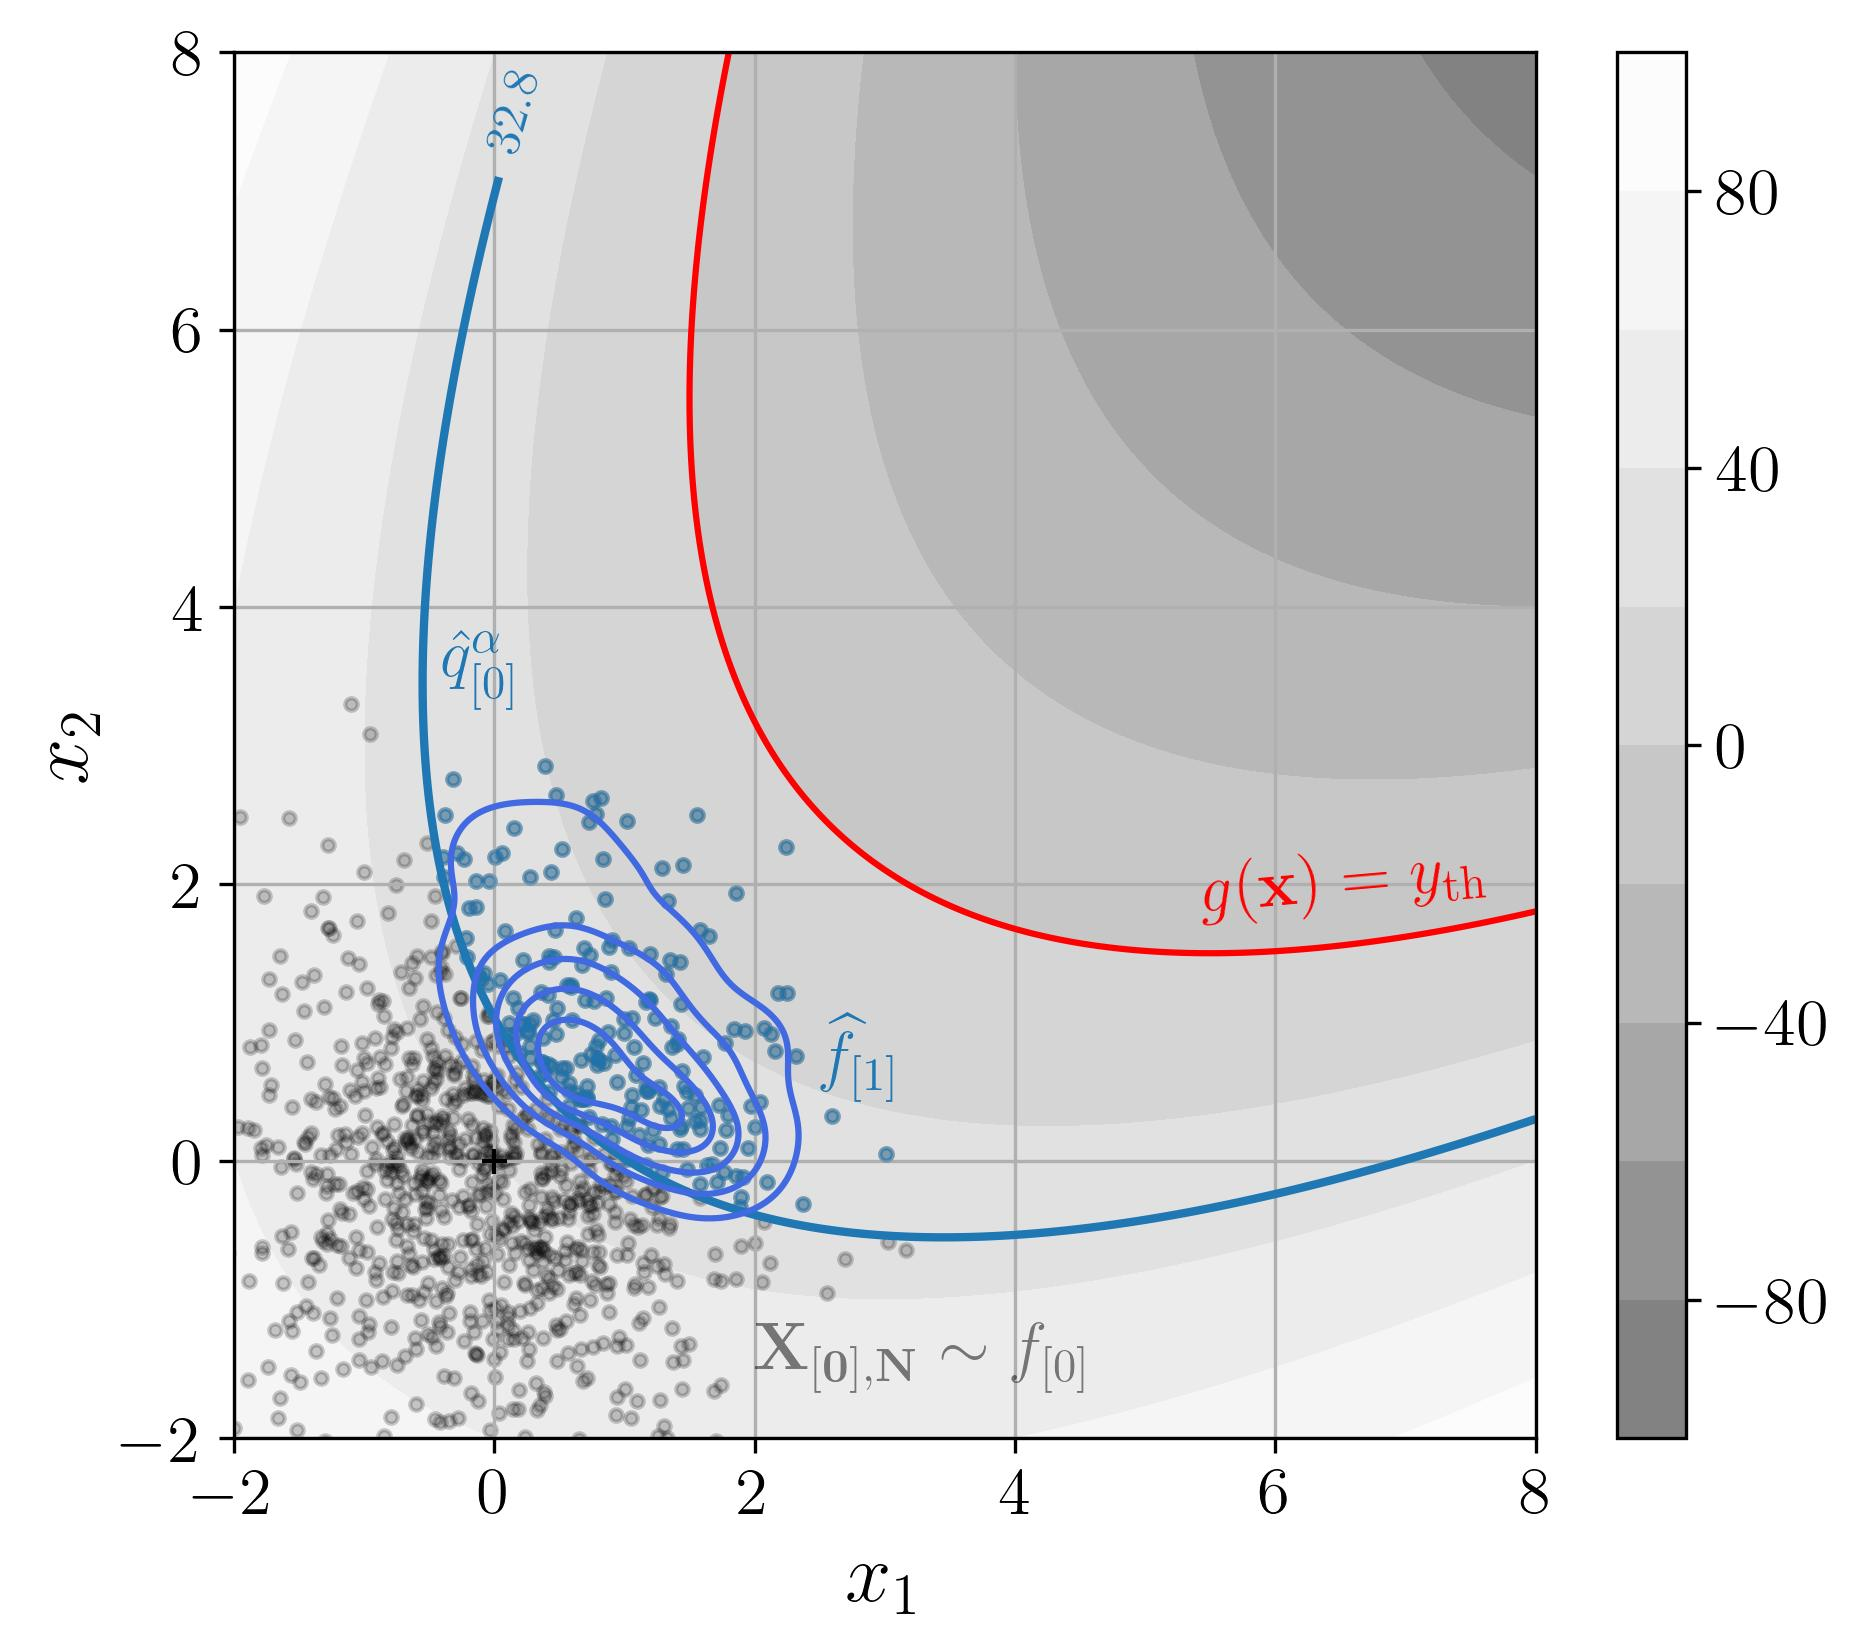
\includegraphics[width=\linewidth]{part3/figures/BANCS/bancs_illustration0.jpg}
        \caption{Iteration $k=0$.}
    \end{subfigure}
    \begin{subfigure}[b]{0.49\linewidth}
        \centering
        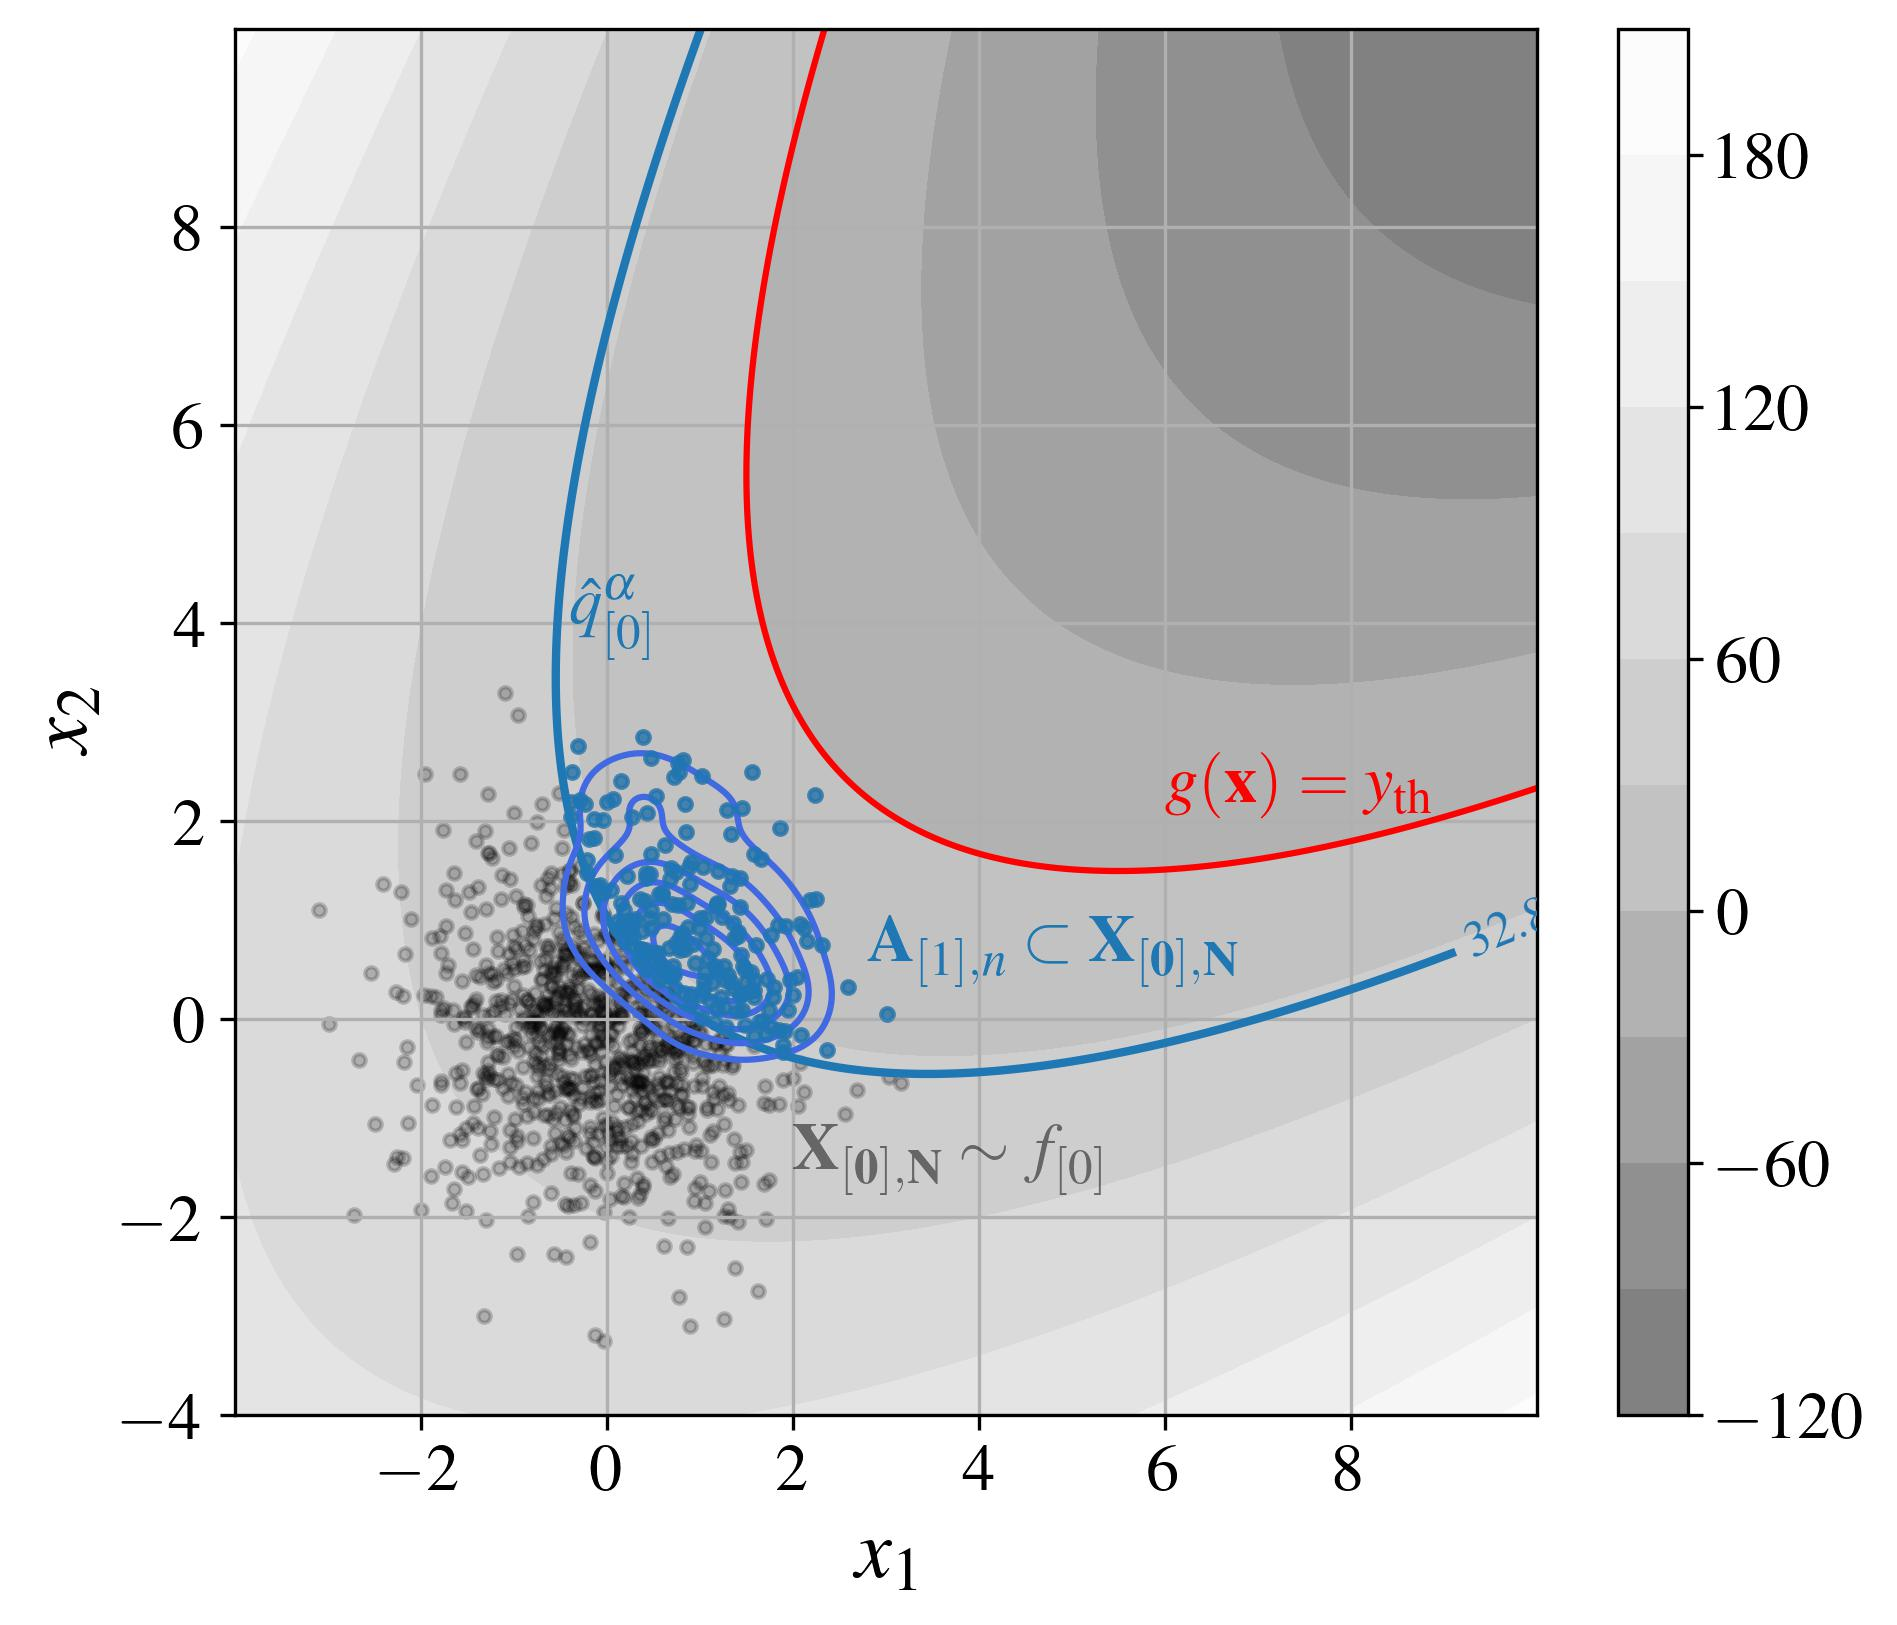
\includegraphics[width=\linewidth]{part3/figures/BANCS/bancs_illustration1.jpg}
        \caption{Iteration $k=1$.}
    \end{subfigure}
    \caption{BANCS algorithm applied to toy-case \#1: illustration of conditional sampling and nonparametric fit at the first and second iterations.}
    \label{fig:bancs_illustration}
\end{figure}
%%%%%%%%%%%%%%%%%%%%%%%%%%%%%%%%%%%%%%%%%%%%%%%%%%%%%%%%%%%%%

Nonparametric inference requires tuning scaling parameters for KDE or a polynomial order $m$ (considered equal in all dimension) for EBC. 
In the current implementation of BANCS, the KDE is tuned using Silverman's rule \citep{silverman_1981} while the EBC is tuned to minimize an asymptotic mean integrated squared error (AMISE). 
As discussed in Chapter~\ref{chpt:3}, for a dataset with size $n$ and dimension $d$, the AMISE tuning for the EBC was defined by \citet{sancetta_satchell_2004} as:
\begin{equation}\label{eq:amise_tuning}
    m_{\mathrm{AIMSE}} = 1 + n^{2/(d+4)}
\end{equation}
In our experience, EBC tuning in \eq{eq:amise_tuning} worked well for the BANCS algorithm and is systematically used in the following. 
This tuning sets a rather low polynomial order to the EBC, which avoids overfitting issues. 
For small sample sizes, e.g., $n<100$, \citet{segers_2017} showed the limits of this tuning. 
However, the typical sample sizes used for rare event estimation should suit the AMISE tuning. 

Ultimately, the estimator of the probability from \eq{eq:failure_proba_c6} is written as a simple IS estimator on the last conditional distribution with PDF $\widehat{f}_{[k_\#]}$:
\begin{equation}
    \widehat{\pf}^{\mathrm{BANCS}} = \frac1N \sum_{i=1}^N \frac{f_\bX(\bx_{[k_\#]}^{(i)})}{\widehat{f}_{[k_\#]}(\bx_{[k_\#]}^{(i)})} \, \1_{\{g(\bx_{[k_\#]}^{(i)}) \leq \yth \}}(\bx_{[k_\#]}^{(i)})\, , \quad \left\{\bx_{[k_\#]}^{(i)}\right\}_{i=1}^N  \overset{\text{i.i.d.}}{\sim} \widehat{f}_{[k_\#]} \, .
\end{equation}
This estimator also benefits from an IS variance, which can also be estimated, using the same sample as previously:
\begin{equation}
    \var(\widehat{\pf}^{\mathrm{BANCS}}) = \frac{1}{N-1} \left[\frac1N \sum_{i=1}^N \left(\frac{f_\bX(\bx_{[k_\#]}^{(i)})}{\widehat{f}_{[k_\#]}(\bx_{[k_\#]}^{(i)})}\right)^2 \, \1_{\{g(\bx_{[k_\#]}^{(i)}) \leq \yth \}}(\bx_{[k_\#]}^{(i)}) \, - \, \left(\widehat{\pf}^{\mathrm{BANCS}}\right)^2\right]
\end{equation}

\fig{fig:bancs_illustration} illustrates the nonparametric fit and conditional sampling in BANCS method on a two-dimensional reliability problem (later introduced as ``toy-case \#1''). 
At the iteration $k=0$, the conditional distribution fitted (with PDF represented by the blue isolines) slightly overlays below the quantile border $\widehat{q}_{[0]}^{p_0}$. 
Ideally, the conditional distribution fitted should be sharp around this border without overfitting the data
At the second iteration, the PDF of the second conditional distribution fitted is represented by the brown isolines. 
This second fit is realized on all the samples above the second quantile $\widehat{q}_{[1]}^{p_0}$, weighted by their respective distribution (see lines 14 and 15 from Algorithm~\ref{alg:bancs}). 
Including the samples from the previous iterations tends to make the fit sharper around the quantile border. 


%Tools to control the goodness of fit of nonparametric conditional distributions are also available. 
%As an example, let us consider the fitted conditional distribution at the first iteration (visible in \fig{fig:bancs_illustration}). 
%Its quantile-quantile plot in \fig{fig:qqplot} shows a good fit of the two marginals by KDE. 
%Then, the goodness of fit of copulas can be evaluated by Kendall's plot, represented in \fig{fig:kendall_plot}. 
%This fit is also good, even if a slight bias is again visible.

%\begin{figure}[!ht]
%    \centering
%    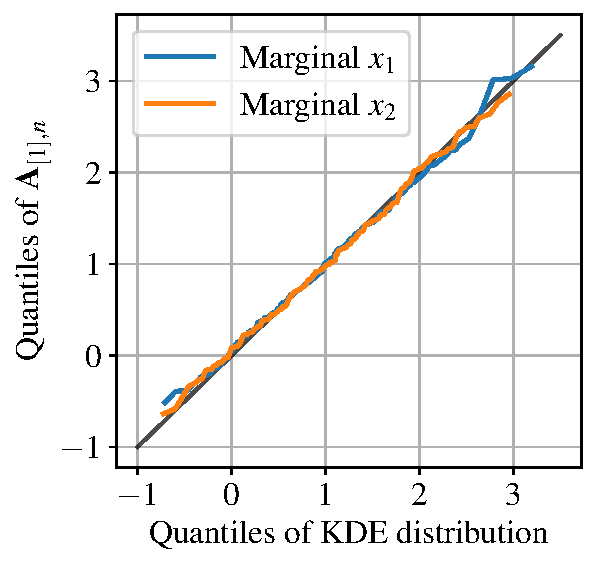
\includegraphics[width=0.6\linewidth]{part3/figures/BANCS/qqplots.pdf}
%    \caption{QQ-plot for KDE of marginals of the conditional distribution from \fig{fig:bancs_illustration}.}
%    \label{fig:qqplot}
%\end{figure}
%
%\begin{figure}[!ht]
%    \centering
%    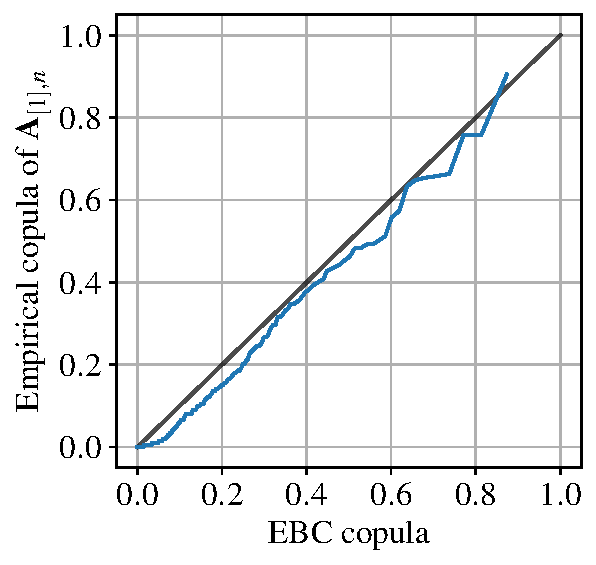
\includegraphics[width=0.6\linewidth]{part3/figures/BANCS/kendall_plot.pdf}
%    \caption{Kendall plot for EBC on the copula of a conditional distribution from \fig{fig:bancs_illustration}.}
%    \label{fig:kendall_plot}
%\end{figure}



%============================================================%
%============================================================%
\section{Numerical experiments}\label{sec:bancs_bench}
%============================================================%
%============================================================%

In the present section, the performances of BANCS algorithm are compared with the ones from subset simulation (SS) and the nonparametric adaptive importance sampling (NAIS). 
The efficiency of SS depends on the choice and tuning of the MCMC algorithm \citep{Papaioannou_PEM_2015}. 
Our work uses the \texttt{OpenTURNS} implementation of the SS\footnotemark (integrating a component-wise Metropolis-Hastings algorithm), 
\footnotetext{SS: \url{https://openturns.github.io/openturns/latest/user_manual/_generated/openturns.SubsetSampling.html}} 
and the \texttt{OpenTURNS} implementation of NAIS\footnotemark. 
\footnotetext{NAIS: \url{https://openturns.github.io/openturns/latest/user_manual/_generated/openturns.NAIS.html}} 
An implementation of the BANCS method and the following numerical experiments are available in a public Git repository\footnote{BANCS: \url{https://github.com/efekhari27/bancs}}. 

In the following analytical numerical experiments, the intermediary probabilities were set to $p_0=0.1$ (following the recommendations from \citet{AuBeck2001}), allowing a fair comparison with subset simulation. 
The size $N$ of each intermediate samples (i.e., subset) evolves in the following set $N\in \{300, 500, 700, 1000, 2000, 5000, 10 000\}$. 
Let us reming that the EBC tuning is setup to minimize the AMISE, such that $m = 1 + n^{\frac{2}{d+4}}$. 
Finally, in order to take into account the variability of the method's results, each experiment is repeated 100 times, allowing the computation of a coefficient of variation $\widehat{\delta} = \frac{\sigma_{\widehat{\pf}}}{\mu_{\widehat{\pf}}}$. 

%============================================================%
\subsection{Analytical toy-cases}
%============================================================%
The reference values of the failure probabilities associated with each problem studied hereafter are obtained by Monte Carlo estimation on very large samples (typically with size $N = 10^9$). 

%------------------------------------------------------------%
\paragraph{Toy-case \#1: Parabolic reliability problem.}
%------------------------------------------------------------%

Let us define the parabolic reliability problem, considering the function $g_1: \R^2 \rightarrow \R$:
\begin{equation}
    g_1(\bx)= (x_1 - x_2) ^ 2 - 8 \, (x_1 + x_2 - 5),
\end{equation}
with the input random vector $\bX = (X_1, X_2)$ following a standard 2-dimensional normal distribution. 
The reliability problem consists in evaluating: $p_{\mathrm{f}, 1} = \mathbb{P} ( g_1(\bX) \leq 0 ) = 1.31 \times 10^{-4}$.

%------------------------------------------------------------%
\paragraph{Toy-case \#2: Four-branch reliability problem.}
%------------------------------------------------------------%

Let us define the four-branch reliability problem (originally proposed by \cite{waarts2000structural}), considering the following function $g_2: \R^2 \rightarrow \R$:
\begin{align}
  g_2(\bx) = \min \begin{pmatrix}
    3+0.1 \, (x_1-x_2)^2-\frac{(x_1+x_2)}{\sqrt{2}}\\
    3+0.1\, (x_1-x_2)^2+\frac{(x_1+x_2)}{\sqrt{2}}\\
    (x_1-x_2)+ \frac{7}{\sqrt{2}}\\
    (x_2-x_1)+ \frac{7}{\sqrt{2}}
  \end{pmatrix}\, ,
\end{align}
with the input random vector $\bX = (X_1, X_2)$ following a standard 2-dimensional normal distribution. 
The reliability problem consists in evaluating: $p_{\mathrm{f}, 2} = \mathbb{P} ( g_2(\bX) \leq 0 ) =  2.22 \times 10^{-3}$.

%------------------------------------------------------------%
\paragraph{Toy-case \#3: Modified Ishigami reliability problem.}
%------------------------------------------------------------%
Let us define the modified Ishigami reliability problem (inspired by \citealp{lemaitre_2015_PLI}), considering the following function $g_3: \R^3 \rightarrow \R$:
\begin{equation}
    g_3(\bx) = \sin(x_1) + 7 \, \sin(x_2)^2 + \frac{x_3^4 \, \sin(x_1)}{10} - 10.5.
\end{equation}
with the input random vector $\bX = (X_1, X_2, X_3)$ following a standard 3-dimensional normal distribution. 
The reliability problem consists in evaluating: $p_{\mathrm{f}, 3} = \mathbb{P} ( g_3(\bX) \leq 0 ) =  1.94 \times 10^{-5}$.

%------------------------------------------------------------%
\paragraph{Toy-case \#4: Medium-dimensional reliability problem.}
%------------------------------------------------------------%

Let us define the medium-dimensional reliability problem (proposed by \citealp{yun2018efficient}), considering the following function $g_4 : \R^7 \rightarrow \R$:

\begin{equation}
    g_4(\bx) = 15.59 \times 10^4 - \frac{x_1 x_3^2}{2 x_3^2} \, \frac{x_2^4 - 4 x_5 x_6 x_7^2 + x_4 (x_6 + 4 x_5 + 2 x_6 x_7)}{x_4 x_5 (x_4 + x_6 + 2 x_6 x_7)},
\end{equation}
with the input random vector $\bX = (X_1, \dots, X_7)$, following a product of normal distributions defined in \cite{yun2018efficient}. 
The reliability problem consists in evaluating: $p_{\mathrm{f}, 4} = \mathbb{P} ( g_4(\bX) \leq 0 ) =  8.10 \times 10^{-3}$.


%------------------------------------------------------------%
\paragraph{Toy-case \#5: Medium-dimensional oscillator problem.}
%------------------------------------------------------------%
Let us define the higher-dimensional oscillator reliability problem (initially introduced by \citealp{destefano_1990}), considering the following function $g_5 : \R^8 \rightarrow \R$:

\begin{equation}
    g_5(\bx) = F_s - 3 k_s \sqrt{\frac{\pi S_0}{4 \zeta_s \omega_s^3} \, \frac{\zeta_a \zeta_s}{\zeta_p \zeta_s (4 \zeta_a^2 + \theta^2) + \gamma \zeta_a^2} \, \frac{\omega_p \, (\zeta_p \omega_p^3 + \zeta_s \omega_s^3)}{4 \zeta_a \omega_a^4}},
\end{equation}
where $\bx = \left(m_p, m_s, k_p, k_s, \zeta_p, \zeta_s, F_s, S_0\right)$,  
$\quad \omega_p=\sqrt{k_p/m_p}, \quad \omega_s=\sqrt{k_s/m_s}, \quad \omega_a = (\omega_p + \omega_s)/2, \quad $
$\zeta_a = (\zeta_p + \zeta_s)/2, \quad \gamma = m_s/m_p, \quad \theta= (\omega_p-\omega_s)/\omega_a$. 
The input random vector $\bX$, defined as a product of marginals following the distributions defined in Table~\ref{tab:oscillator}. 
The reliability problem consists in evaluating: $p_{\mathrm{f}, 5} = \mathbb{P} ( g_5(\bX) \leq 0 ) =  3.78 \times 10^{-7}$.
A representation of this high-dimensional function in \fig{fig:crosscut_oscillator} shows its cross-sections by pairs of inputs passing through FORM's design point $P^*$. 
Such visualization allows to perceive the nonlinearity of the problem near the design point. 
Note that the color scale associated to the output values is log-transformed to increase the color gradient at the border of the failure domain. 


\begin{table}[h]
\centering
\begin{tabular}{ lcccccccc }
    \hline
    Variable            & $m_p$ & $m_s$ & $k_p$ & $k_s$ & $\zeta_p$ & $\zeta_s$ & $F_s$ & $S_0$ \\
    \hline          
    Distribution        &  \multicolumn{8}{c}{Lognormal} \\ 
    Mean                & 1.5 & 0.01 & 1.0 & 0.01 & 0.05 & 0.02 & 27.5 & 100.0\\ 
    Coeff. of variation & 0.1 & 0.1 & 0.2 & 0.2 & 0.4 & 0.5 & 0.1 & 0.1\\
    \hline
\end{tabular}
\caption{Random inputs from the toy-case \#5.}
\label{tab:oscillator}
\end{table}

%============================================================%
\subsection{Benchmark results and analysis}
%============================================================%

In the present section, the BANCS algorithm is applied to three analytical toy-cases and its performances are compared with SS and NAIS. 
After representing the two first iterations of BANCS on toy-case \#1 in \fig{fig:bancs_illustration}, all BANCS iterations from this case are illustrated in \fig{fig:2D_toycase_reliability} (a). 
This figure shows the intermediate quantiles $\{\widehat{q}_{[k]}^{p_0}\}_{k=1}^{k_\#}$ which are estimated over conditional samples of size $N=10^4$. 
The points of each sample exceeding their respective $p_0$-quantile are also represented in the same color as their $p_0$-quantile border. 
\fig{fig:2D_toycase_reliability} (b) provides the same kind of illustration for BANCS applied to test-case \#2, a well-known system problem. 
On these two-dimensional cases, one can visualize the empirical quantiles driving the conditional distributions towards the failure domain(s), and the ability of the nonparametric inference to capture multi-modal patterns.  

After this first illustration of BANCS, a more extensive benchmark is proposed. 
To present a fair assessment the estimators' dispersion, each experiment is independently repeated $100$ times. 
Then, a Boostrap procedure on this set allows to compute a confidence interval of the mean failure probability. 
Empirical variances and coefficients of variation (COV) associated with the probability estimators are also computed on the sets of repetitions. 
This way, the SS coefficient of variation is not the result of an approximation (tending to underestimate the true SS coefficient of variation \citealp{Papaioannou_PEM_2015}).
\fig{fig:bancs_benchmark} summarizes the results of this benchmark comparing BANCS with SS and NAIS for different sample sizes $N \in \{300,\, 500,\, 700,\, 10^3,\, 2\cdot10^3,\, 5\cdot10^3,\, 10^4\}$.  
On the left side, the estimates of failure probabilities repeated 100 times are displayed by their average over the repetitions (full lines) and their Bootsrap confidence intervals. 
The reference value for each problem is also represented by a horizontal black line. 
On the right side, an estimate of the coefficient of variation provides a normalized information on the dispersion of the estimators.  
Note that all the estimates are plotted against their total number of samples (corresponding to the number of evaluations to the function). 

To present a diverse panel of problems, the benchmark is conducted on test-case \#2 (four-branch problem with $d=2$), test-case \#4 (with $d=7$), test-case \#5 (oscillator problem with $d=8$). 
BANCS consistently showed good results on all three cases. 
The variance of its estimator is always smaller or equivalent to the SS variance. 
In test-cases \#2 and \#3, BANCS estimation converges faster than SS and as fast as NAIS. 
For test-case \#4, the NAIS implementation used does not support input distributions with bounded domains and was therefore removed. 
BANCS did not encounter the same difficulty as it fits separately the copula and the marginals (which can be easily truncated). 
On this rare and complex case (notice the nonlinearity in the cross-cut in \fig{fig:crosscut_oscillator}), SS is more accurate for small-sized samples (i.e., $N\leq 10^3$) but becomes equivalent to BANCS for larger sample sizes. 
In general, BANCS showed equivalent or better performances than SS and NAIS (on these first cases), while providing i.i.d. sampling and the flexibility of nonparametric inference.   

\begin{figure}
    \centering
    \begin{subfigure}[b]{0.49\linewidth}
        \centering
        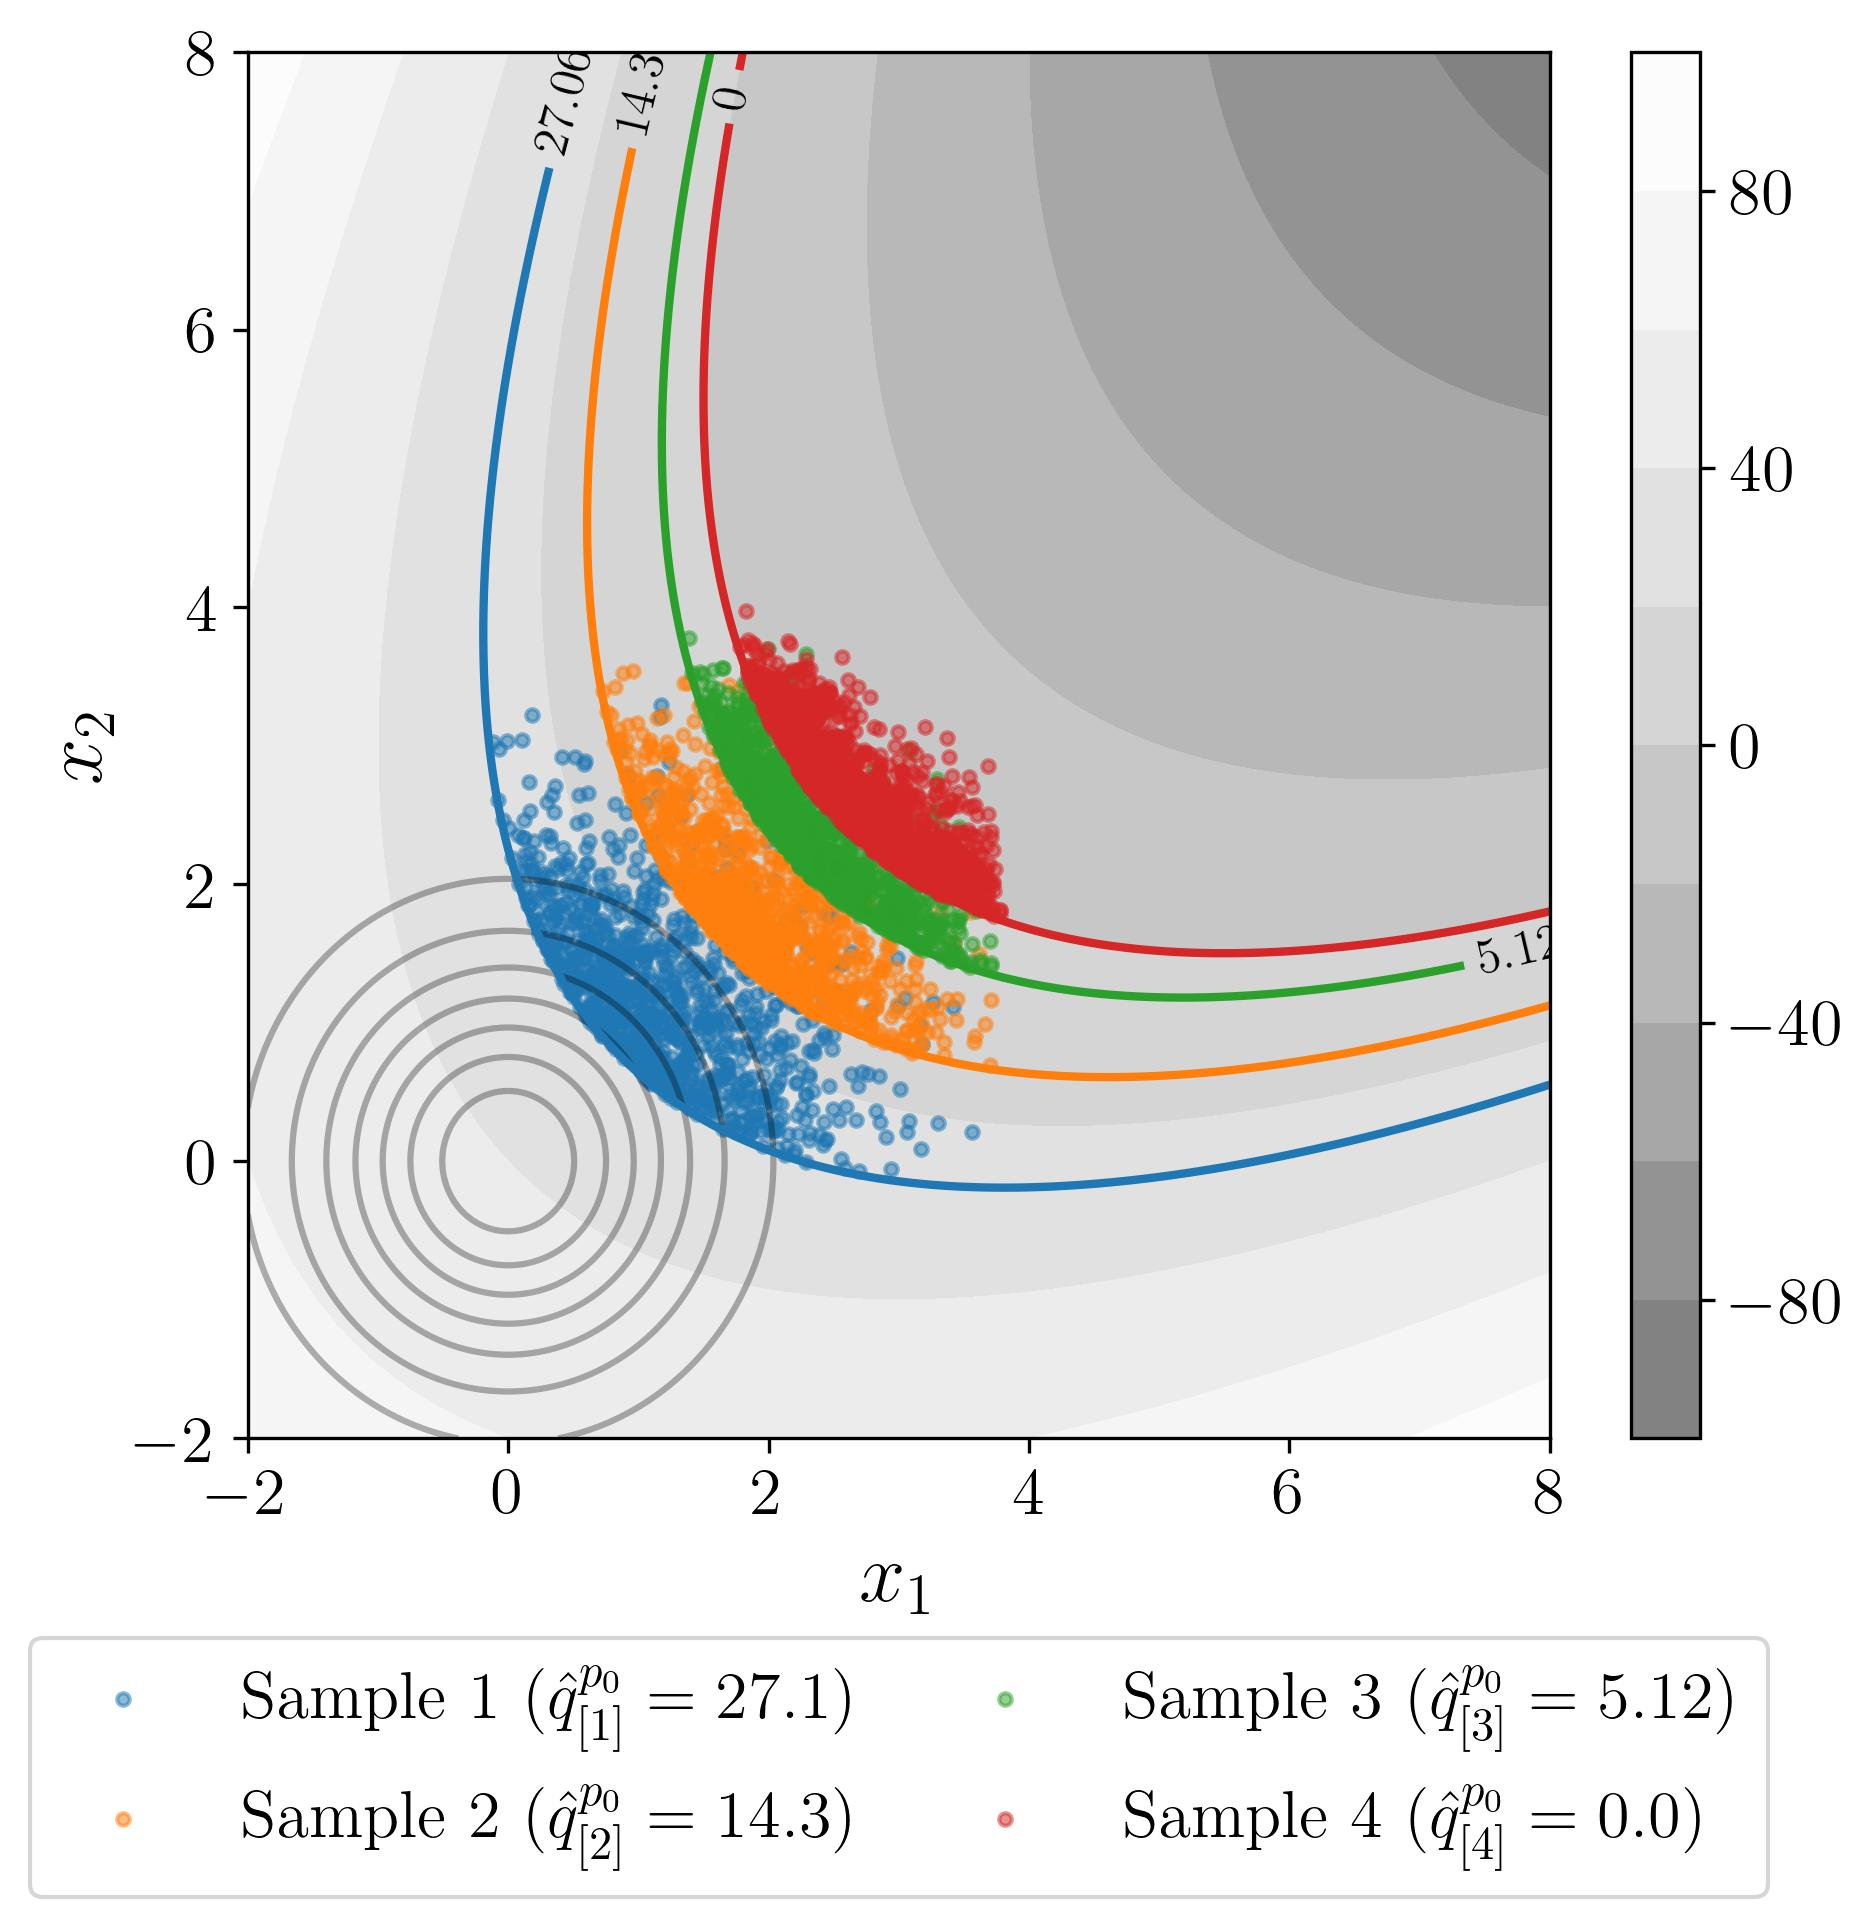
\includegraphics[width=\linewidth]{part3/figures/BANCS/bancs_parabolic.jpg}
        \caption{Toy-case \#1.}
    \end{subfigure}
    \begin{subfigure}[b]{0.49\linewidth}
        \centering
        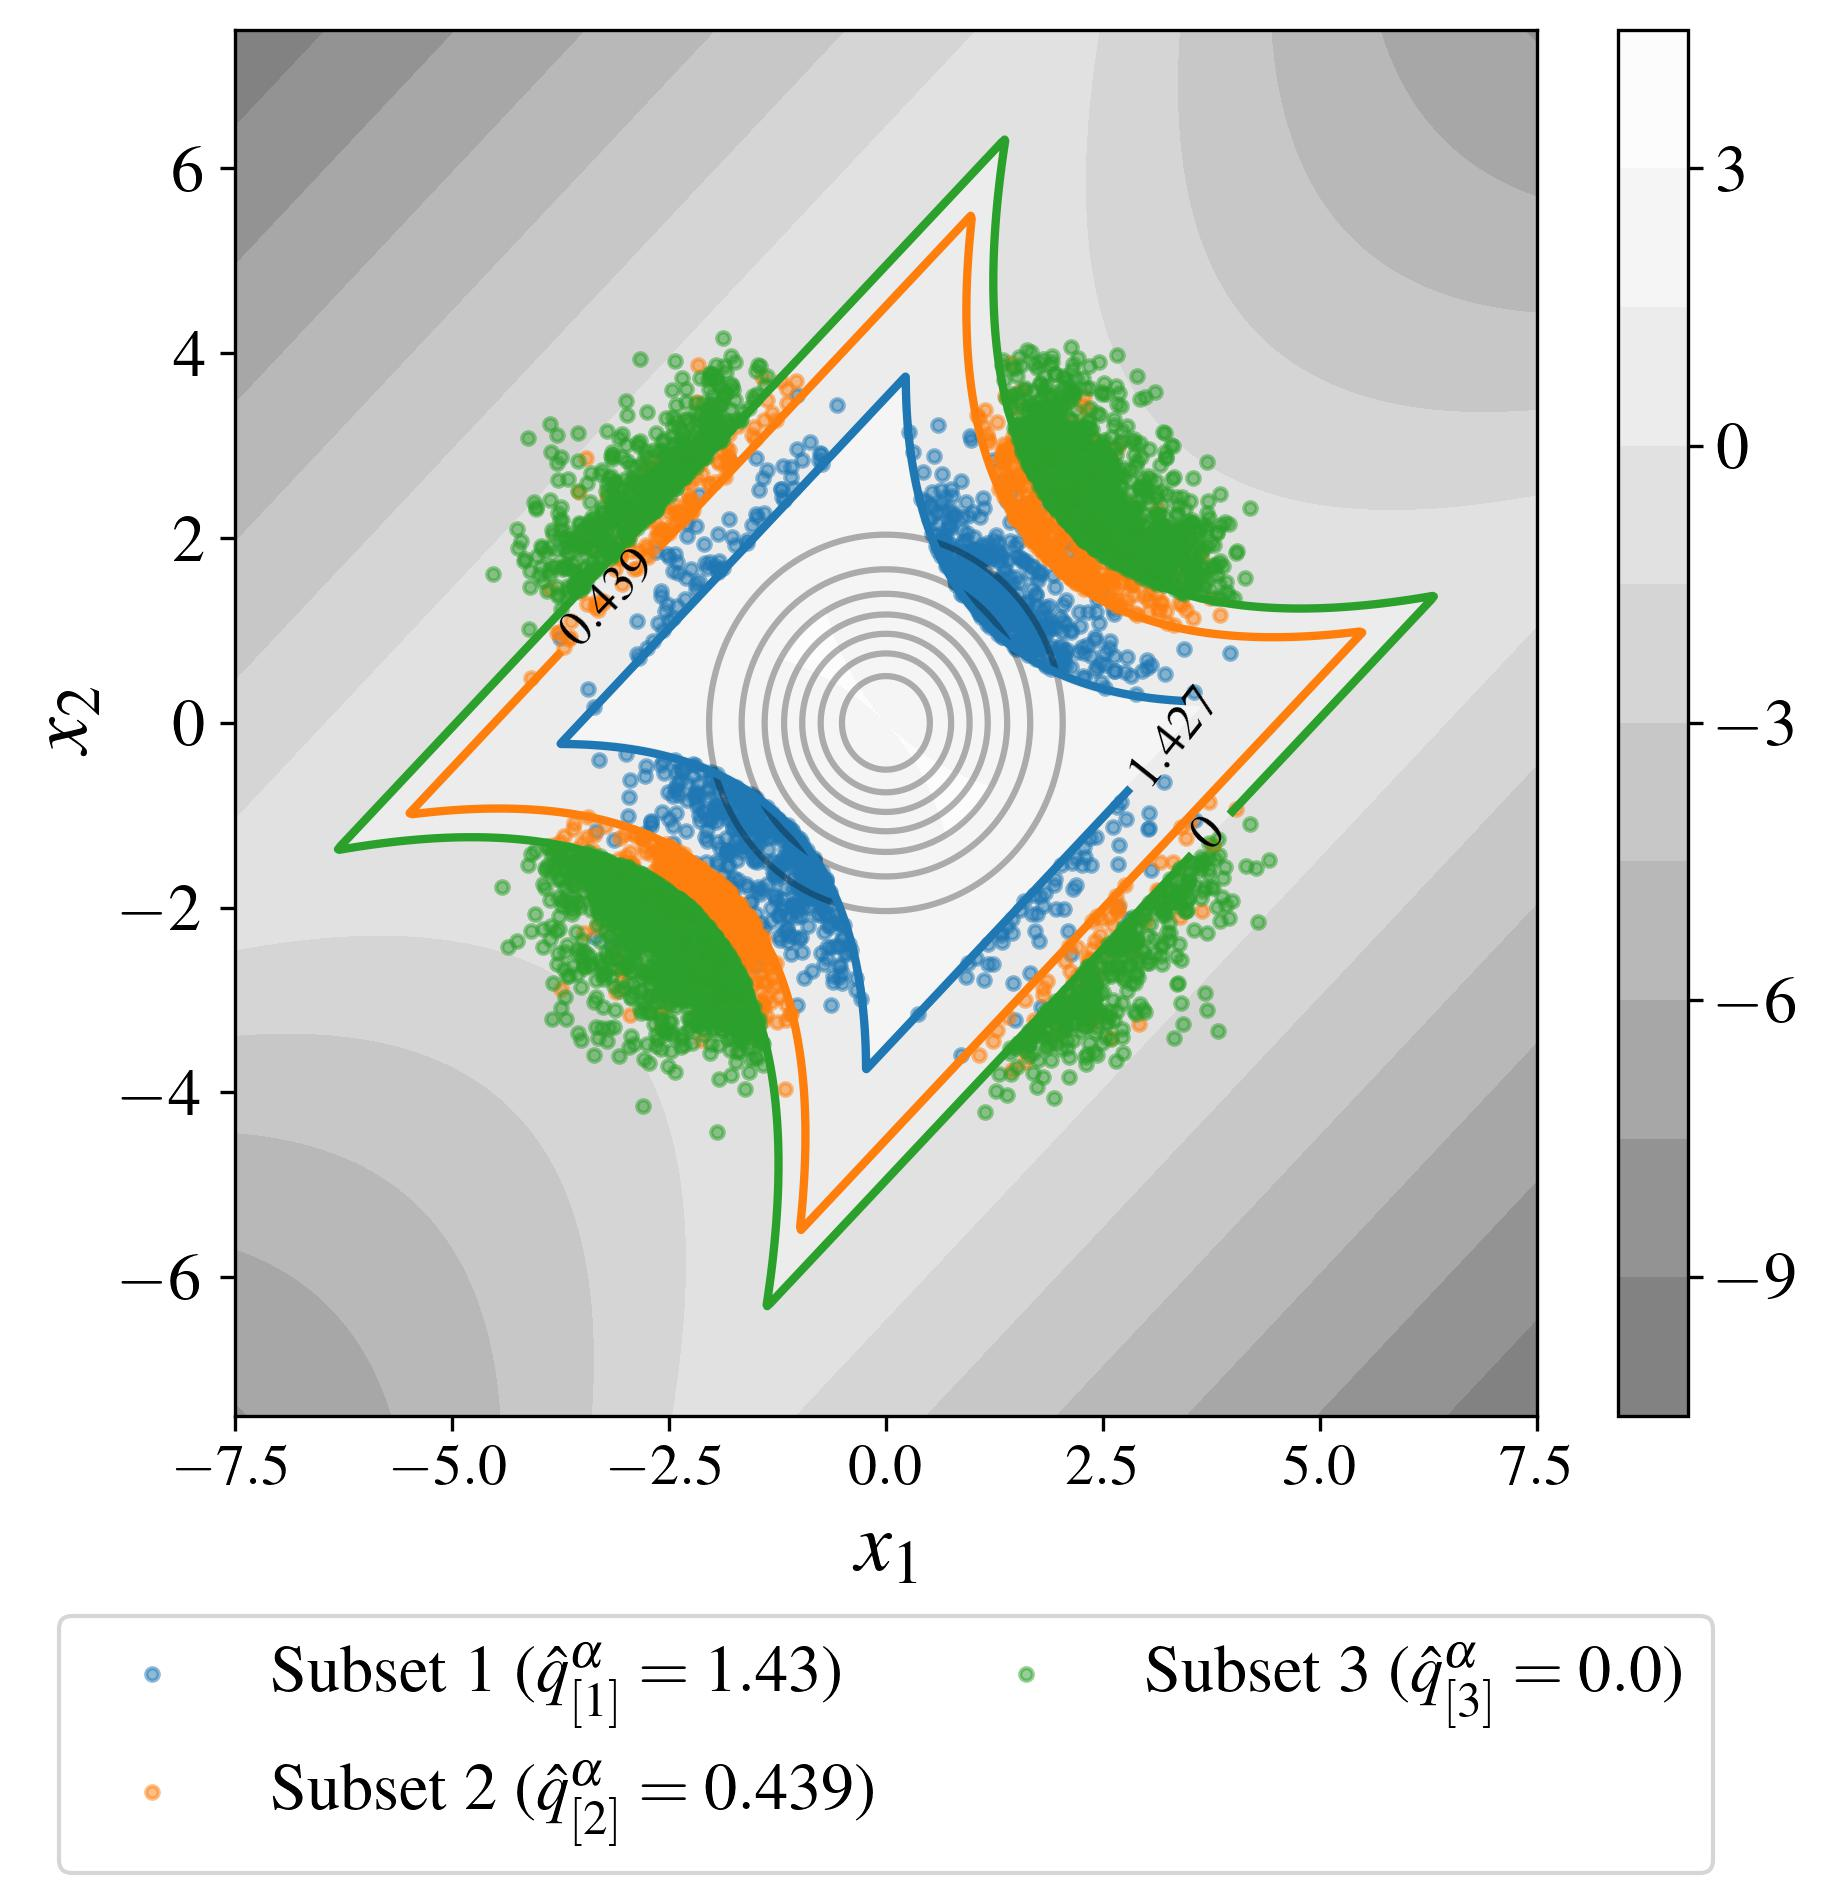
\includegraphics[width=\linewidth]{part3/figures/BANCS/bancs_4branch.jpg}
        \caption{Toy-case \#2.}
    \end{subfigure}
    \caption{BANCS iterations on the two-dimensional reliability problems (for $N=10^4$ and $p_0=0.1$). 
    Only the samples exceeding the intermediary thresholds are represented.}
    \label{fig:2D_toycase_reliability}
\end{figure}


\begin{figure}
    \centering
    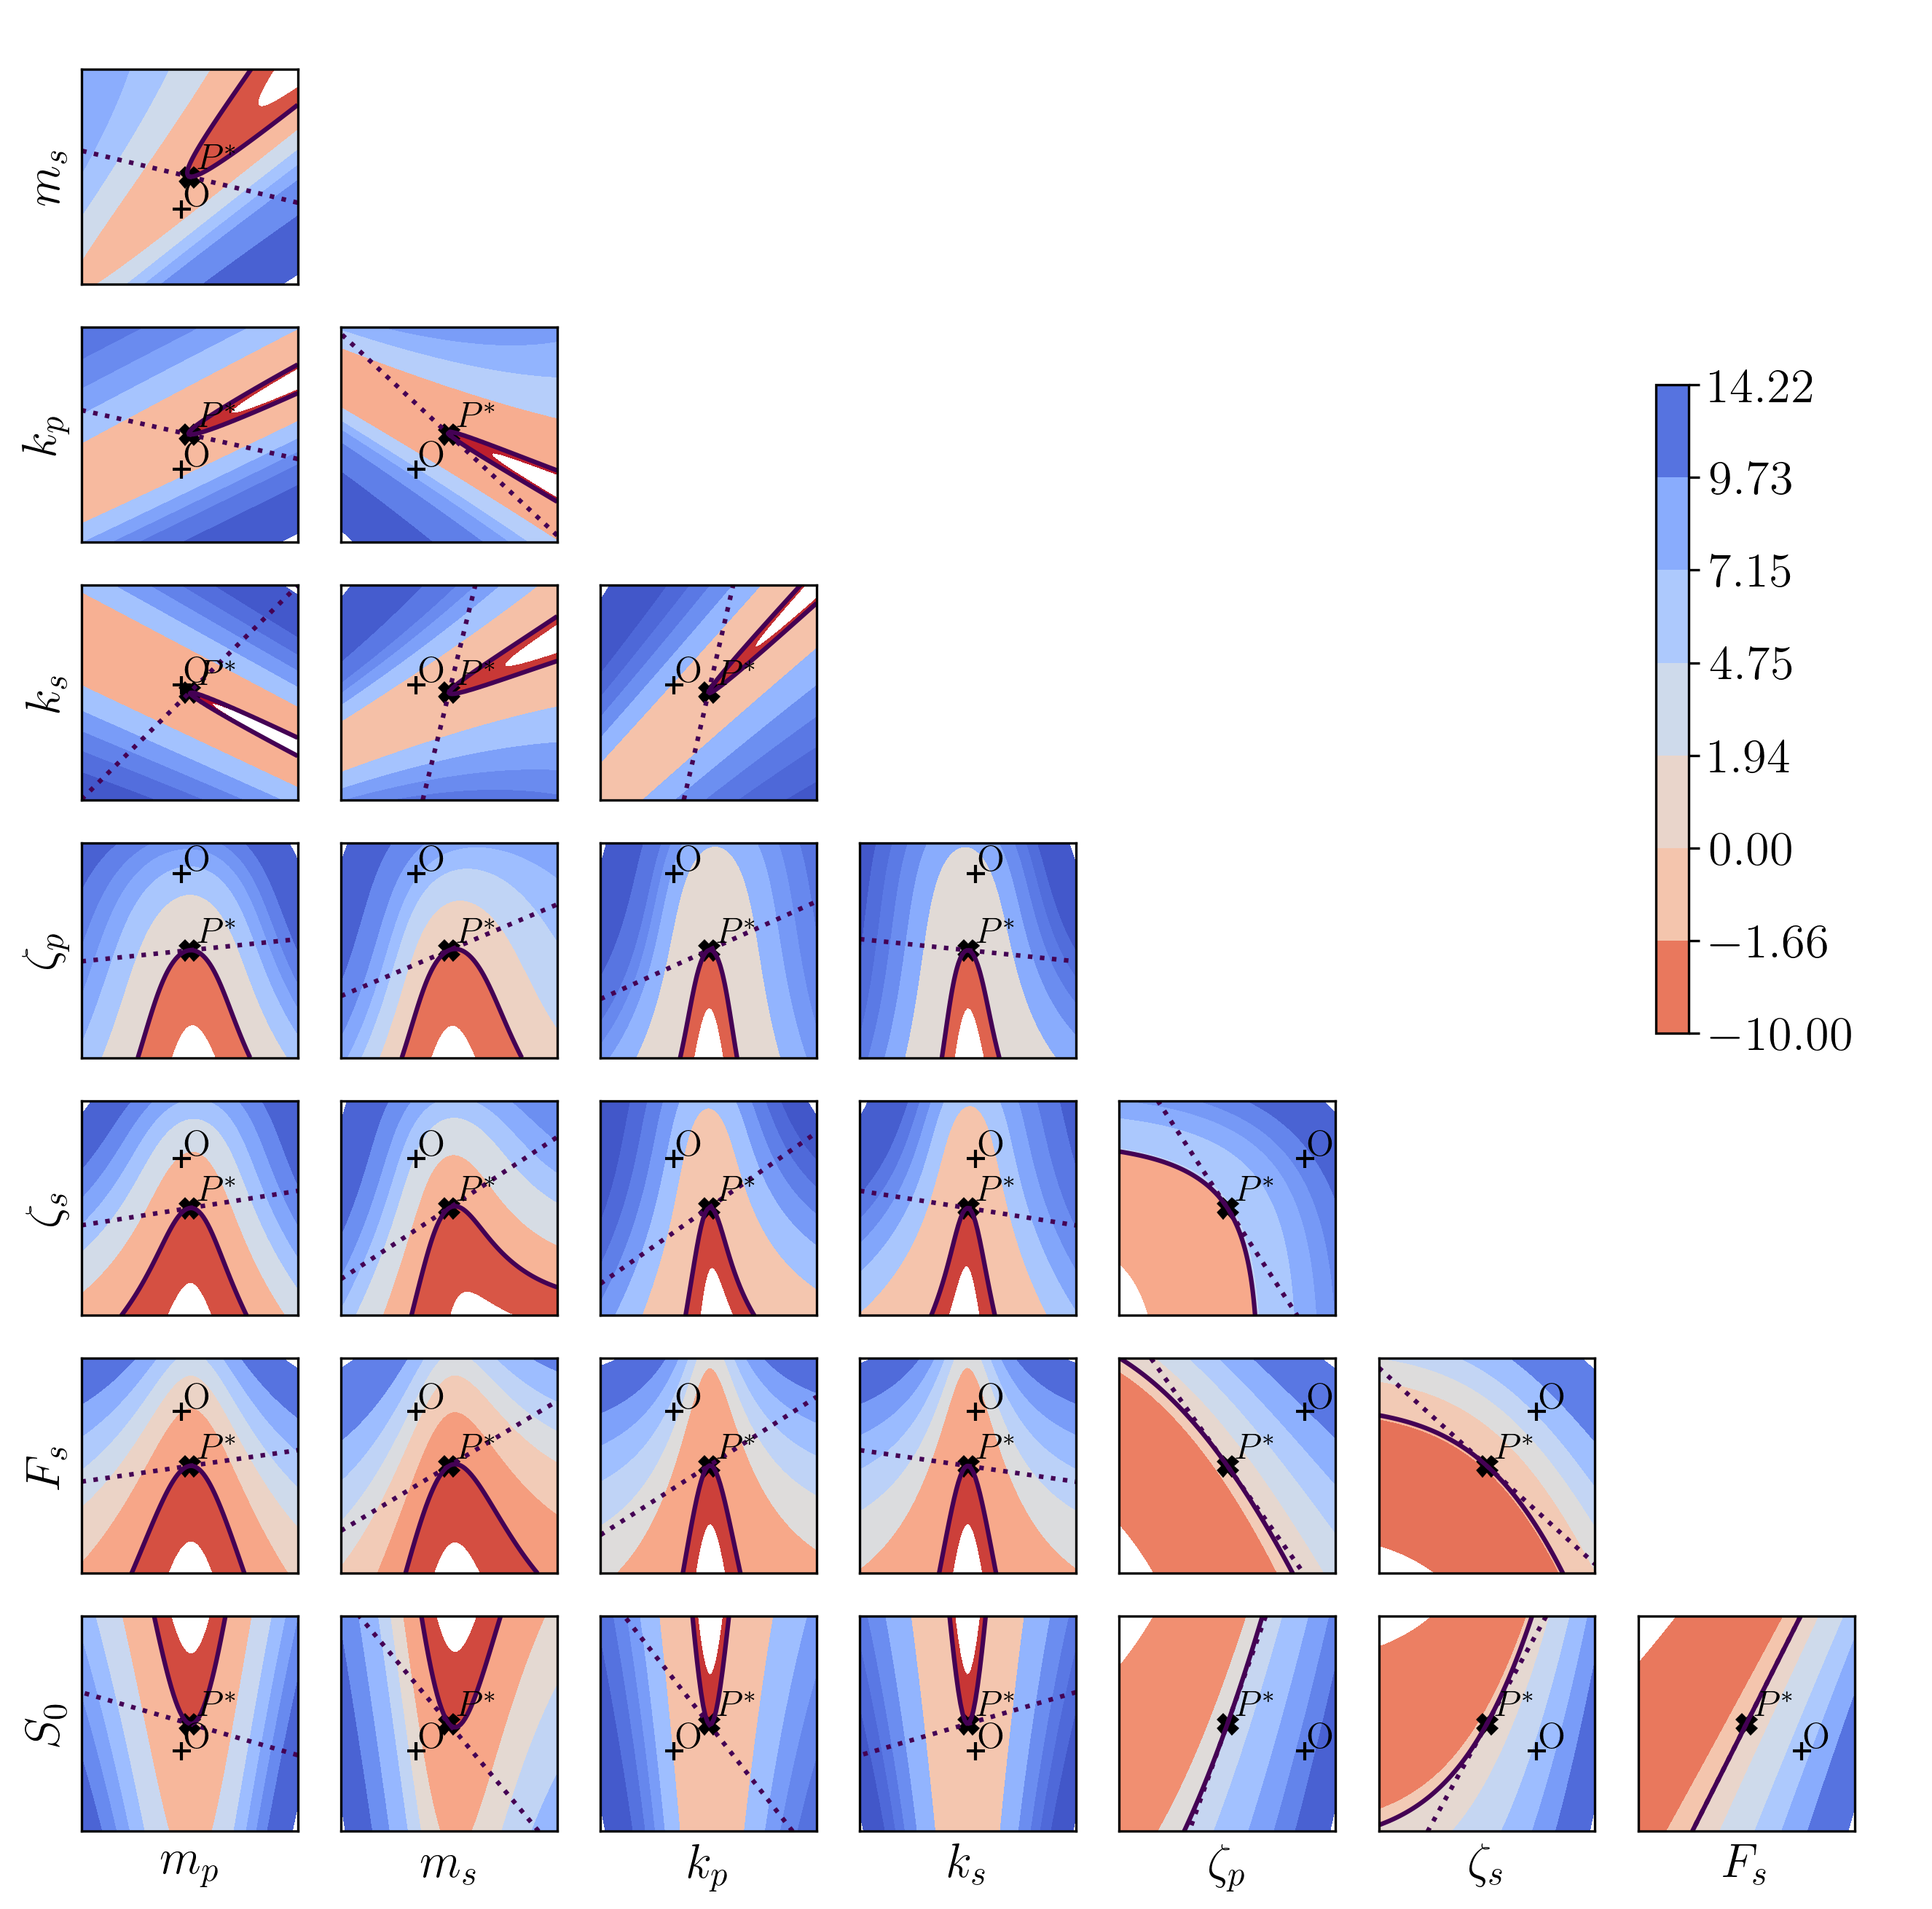
\includegraphics[width=0.7\textwidth]{part3/figures/BANCS/crosscut_oscillator.png}
    \caption{Cross-cut visualization of the function of test-case \#5 through FORM's most-probable failure point $P^*$. 
    The limit-state function (full line) delimits the safe domain (in blue) and the failure domain (in red). 
    FORM produces the Taylor approximation around $P^*$ (dashed lines).}
    \label{fig:crosscut_oscillator}
\end{figure}


\begin{figure}
    \centering
    \begin{subfigure}[b]{0.49\linewidth}
        \centering
        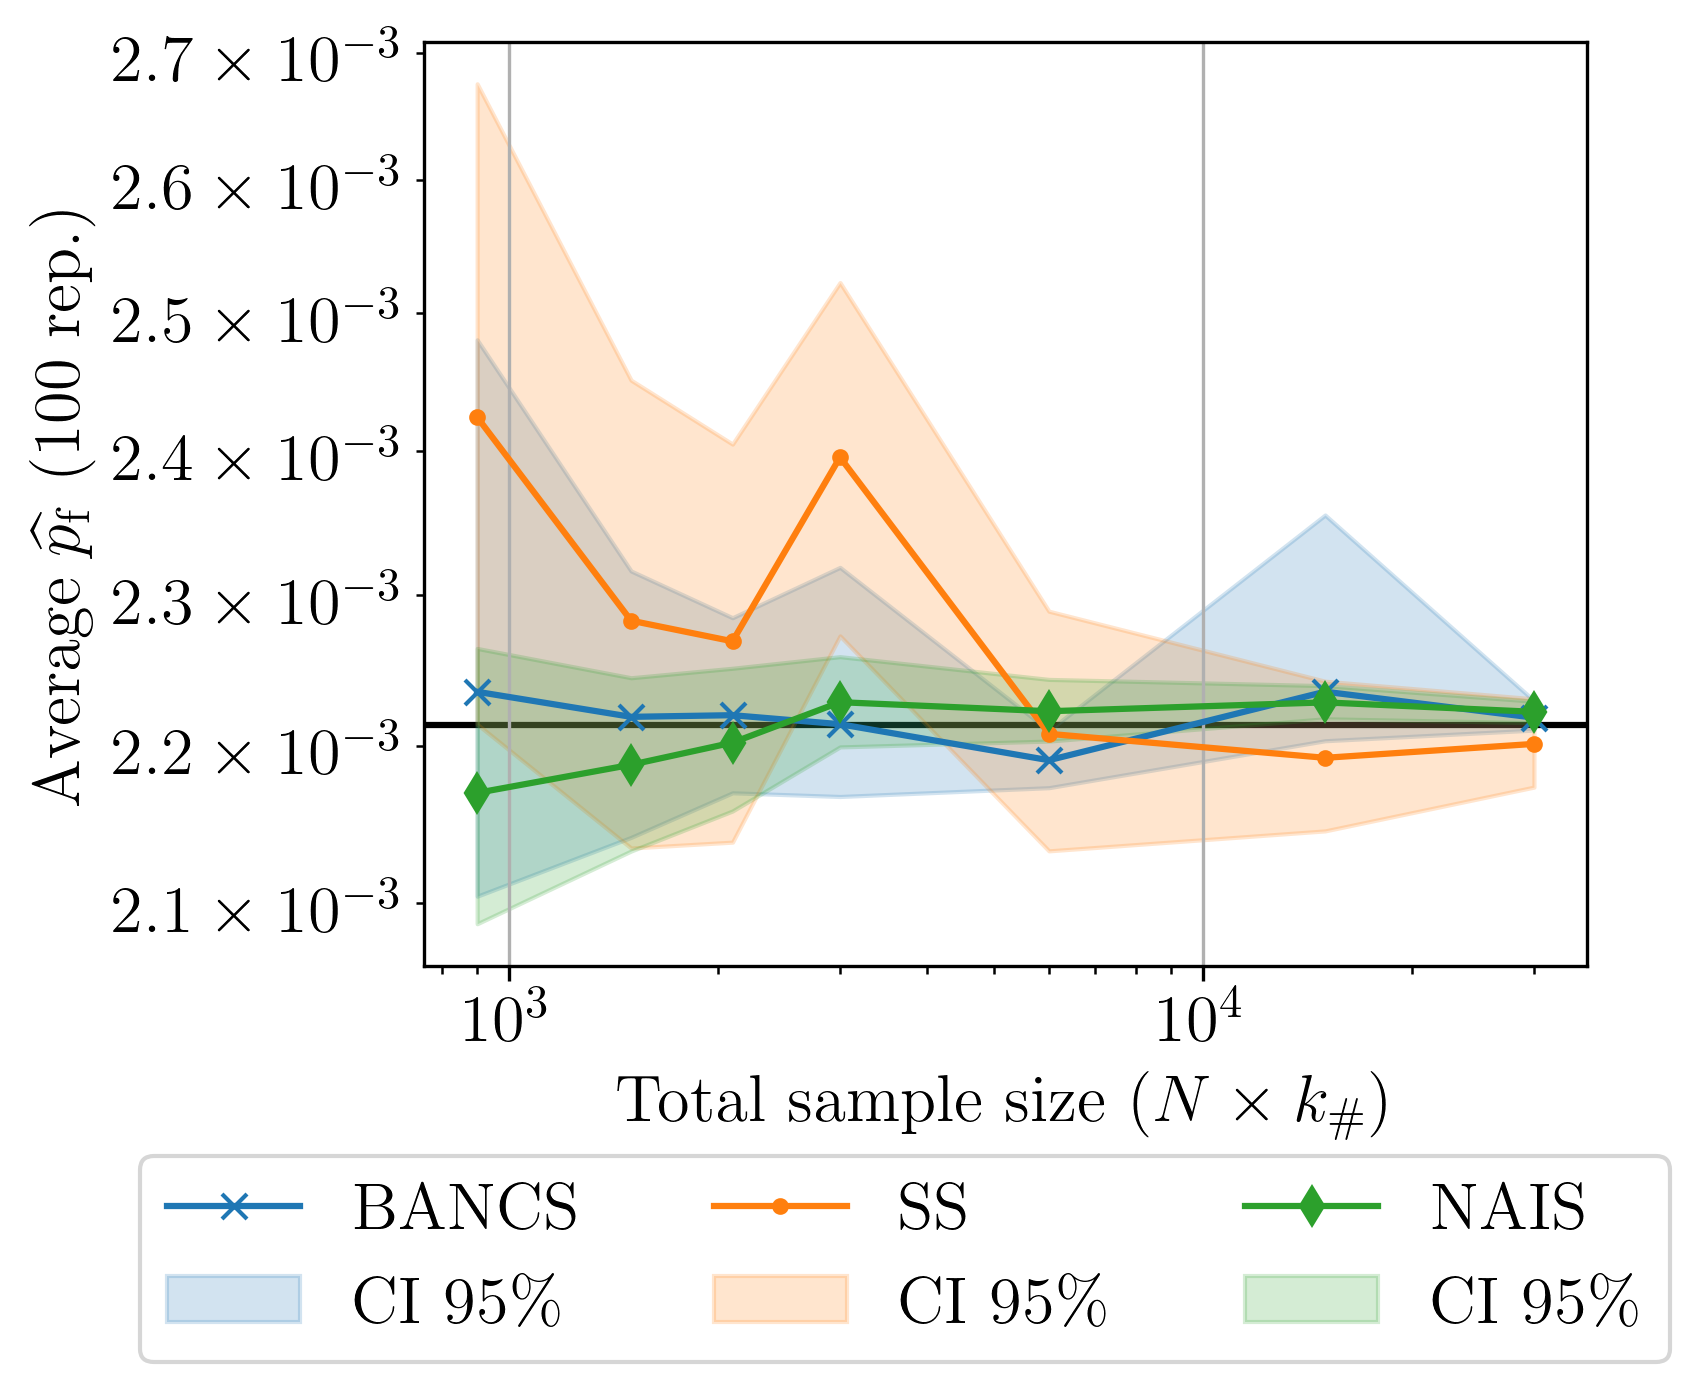
\includegraphics[width=\linewidth]{part3/figures/BANCS/RP4B_mean.png}
        \caption{Failure probability (toy-case \#2).}
    \end{subfigure}
    \begin{subfigure}[b]{0.47\linewidth}
        \centering
        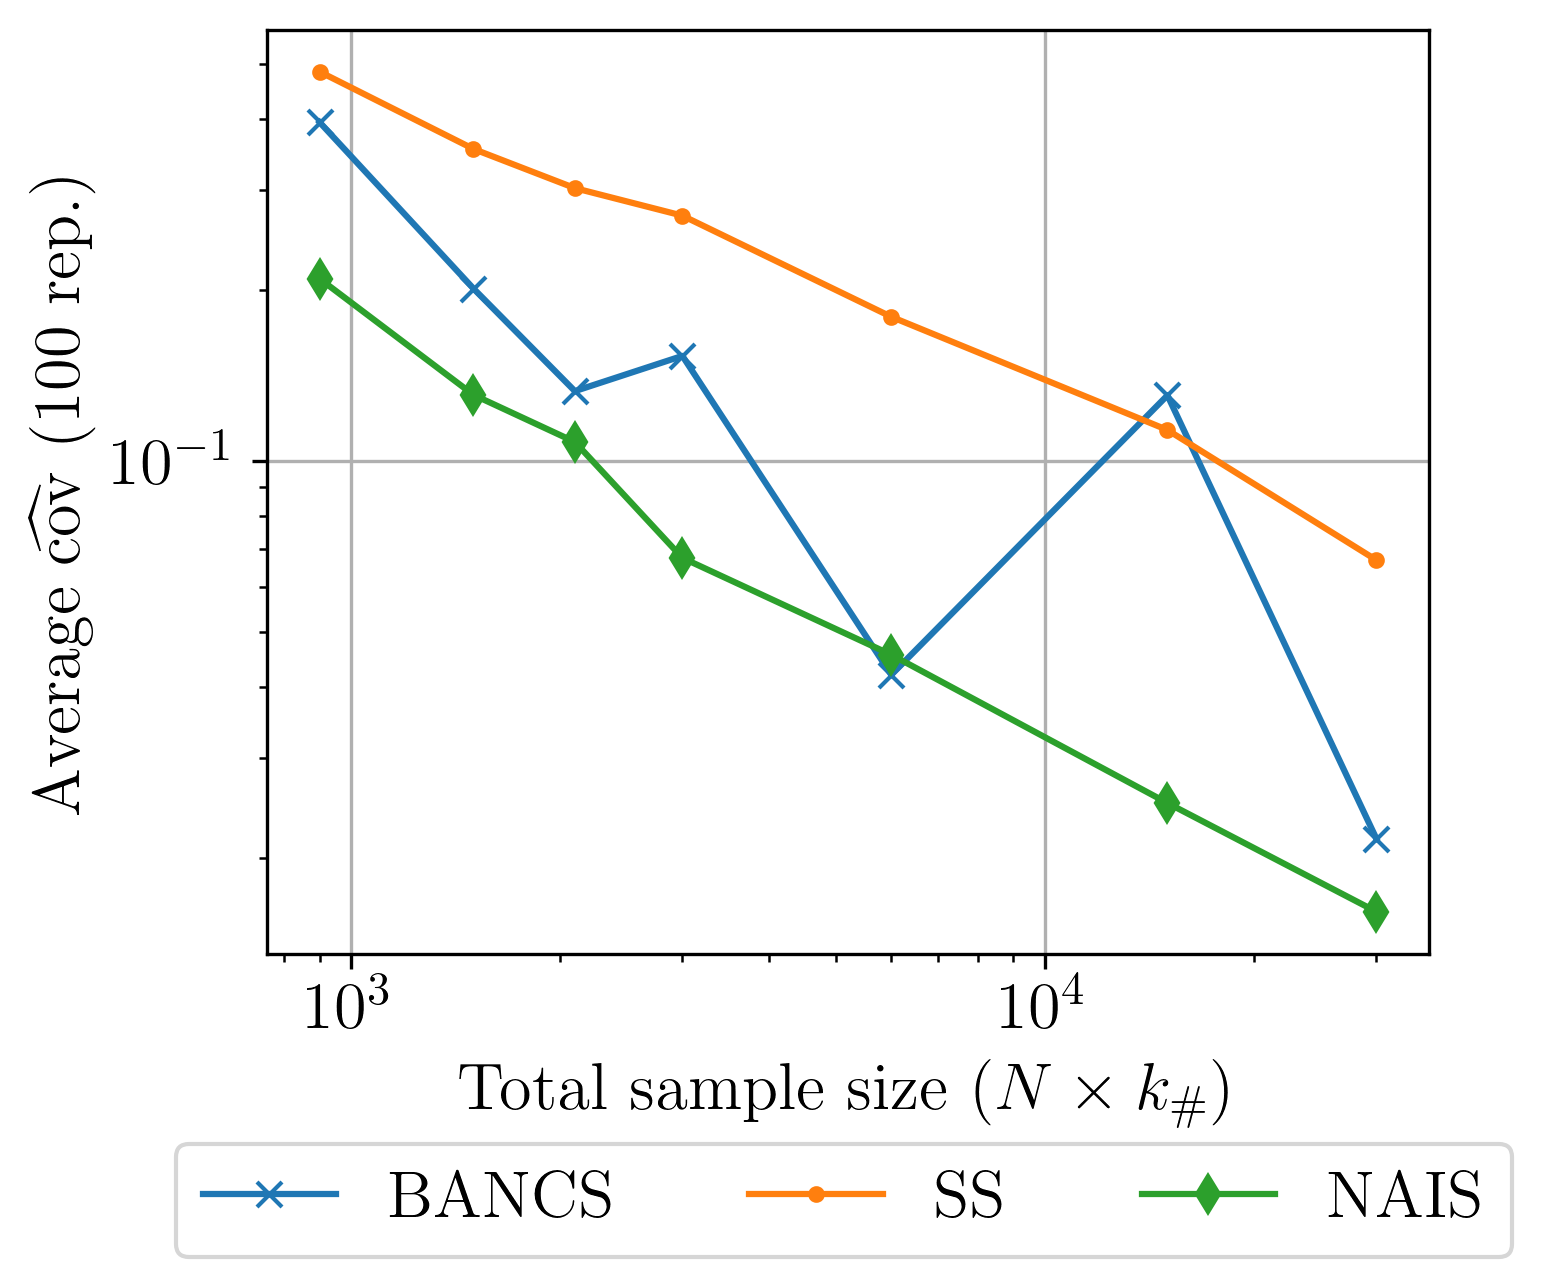
\includegraphics[width=\linewidth]{part3/figures/BANCS/RP4B_cov.png}
        \caption{Coefficient of variation (toy-case \#2).}
    \end{subfigure}
    \begin{subfigure}[b]{0.49\linewidth}
        \centering
        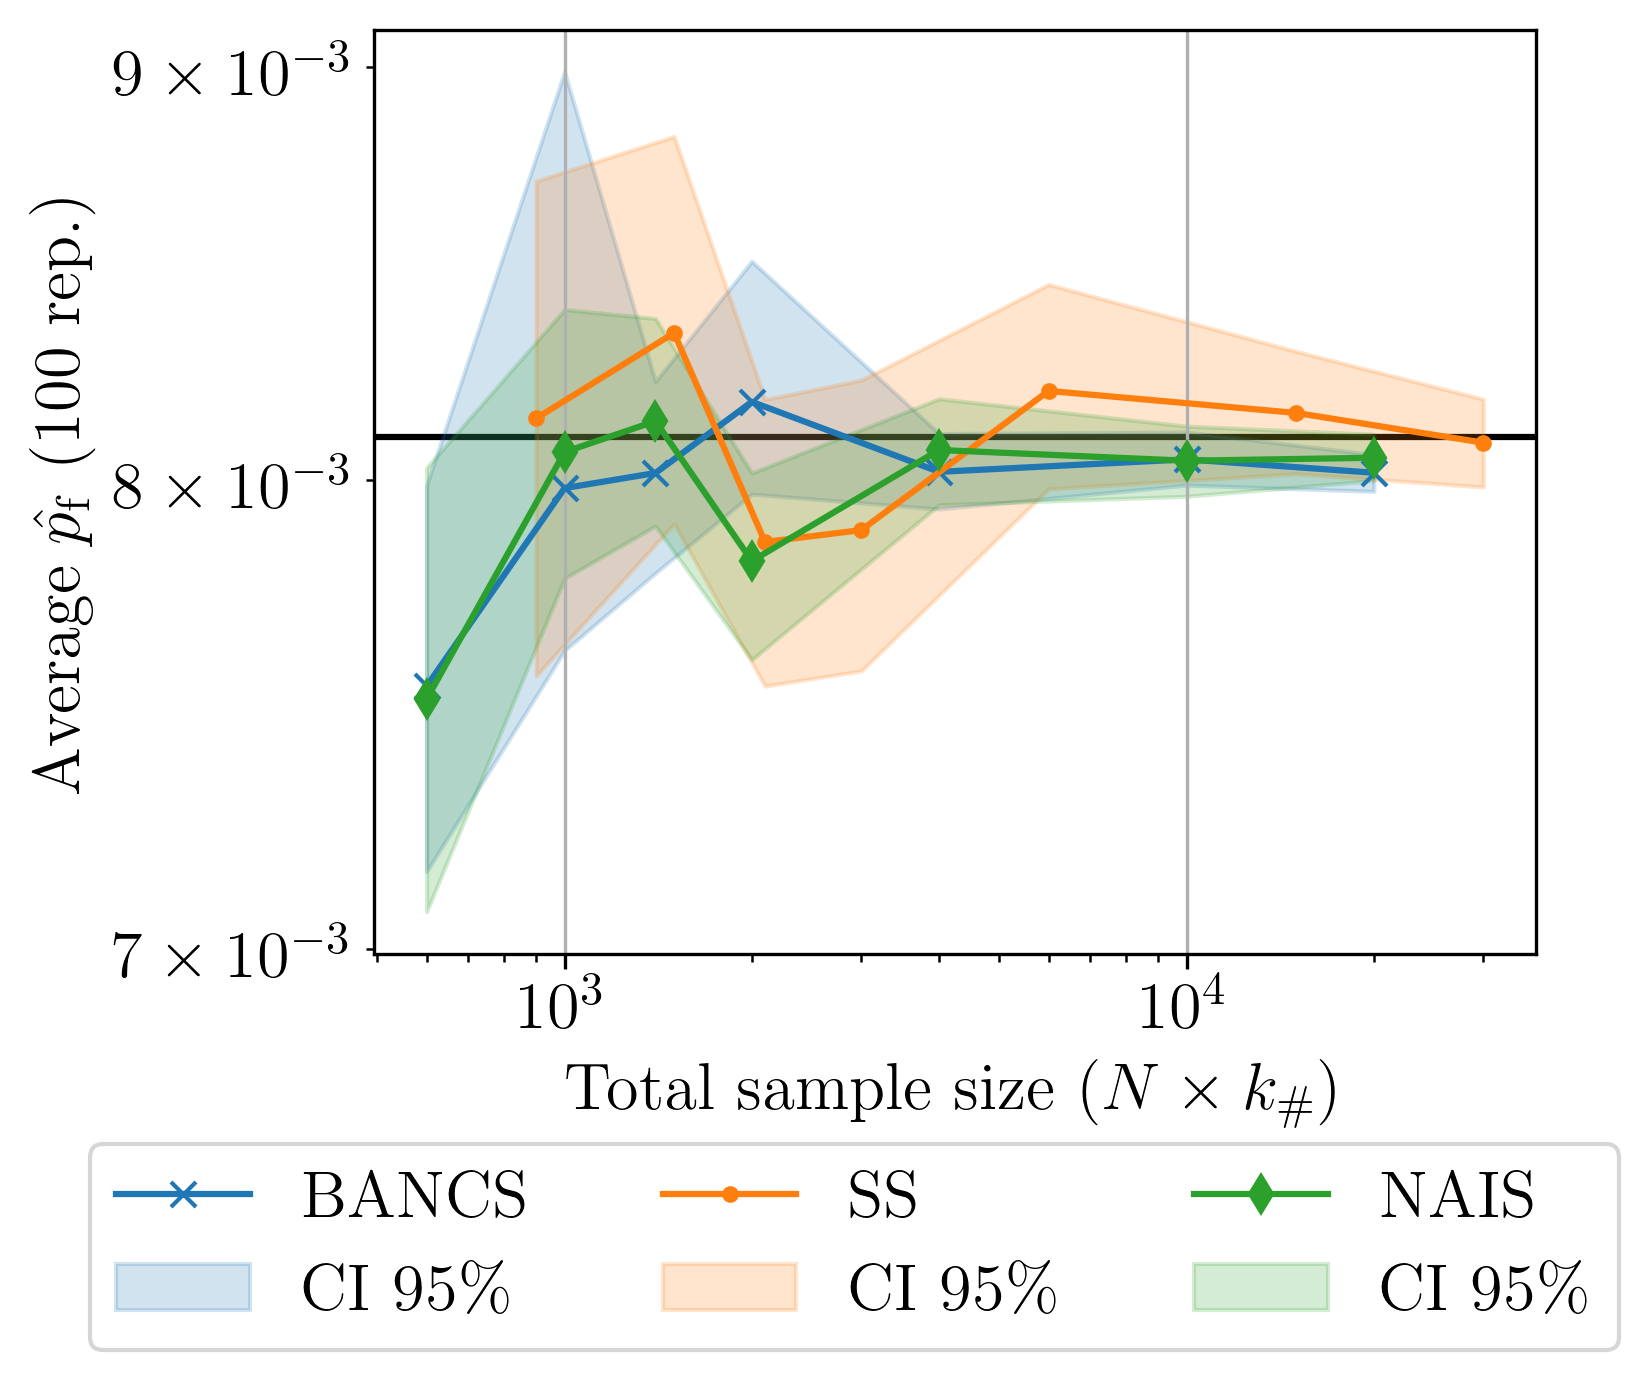
\includegraphics[width=\linewidth]{part3/figures/BANCS/RP38_mean.png}
        \caption{Failure probability (toy-case \#4).}
    \end{subfigure}
    \begin{subfigure}[b]{0.47\linewidth}
        \centering
        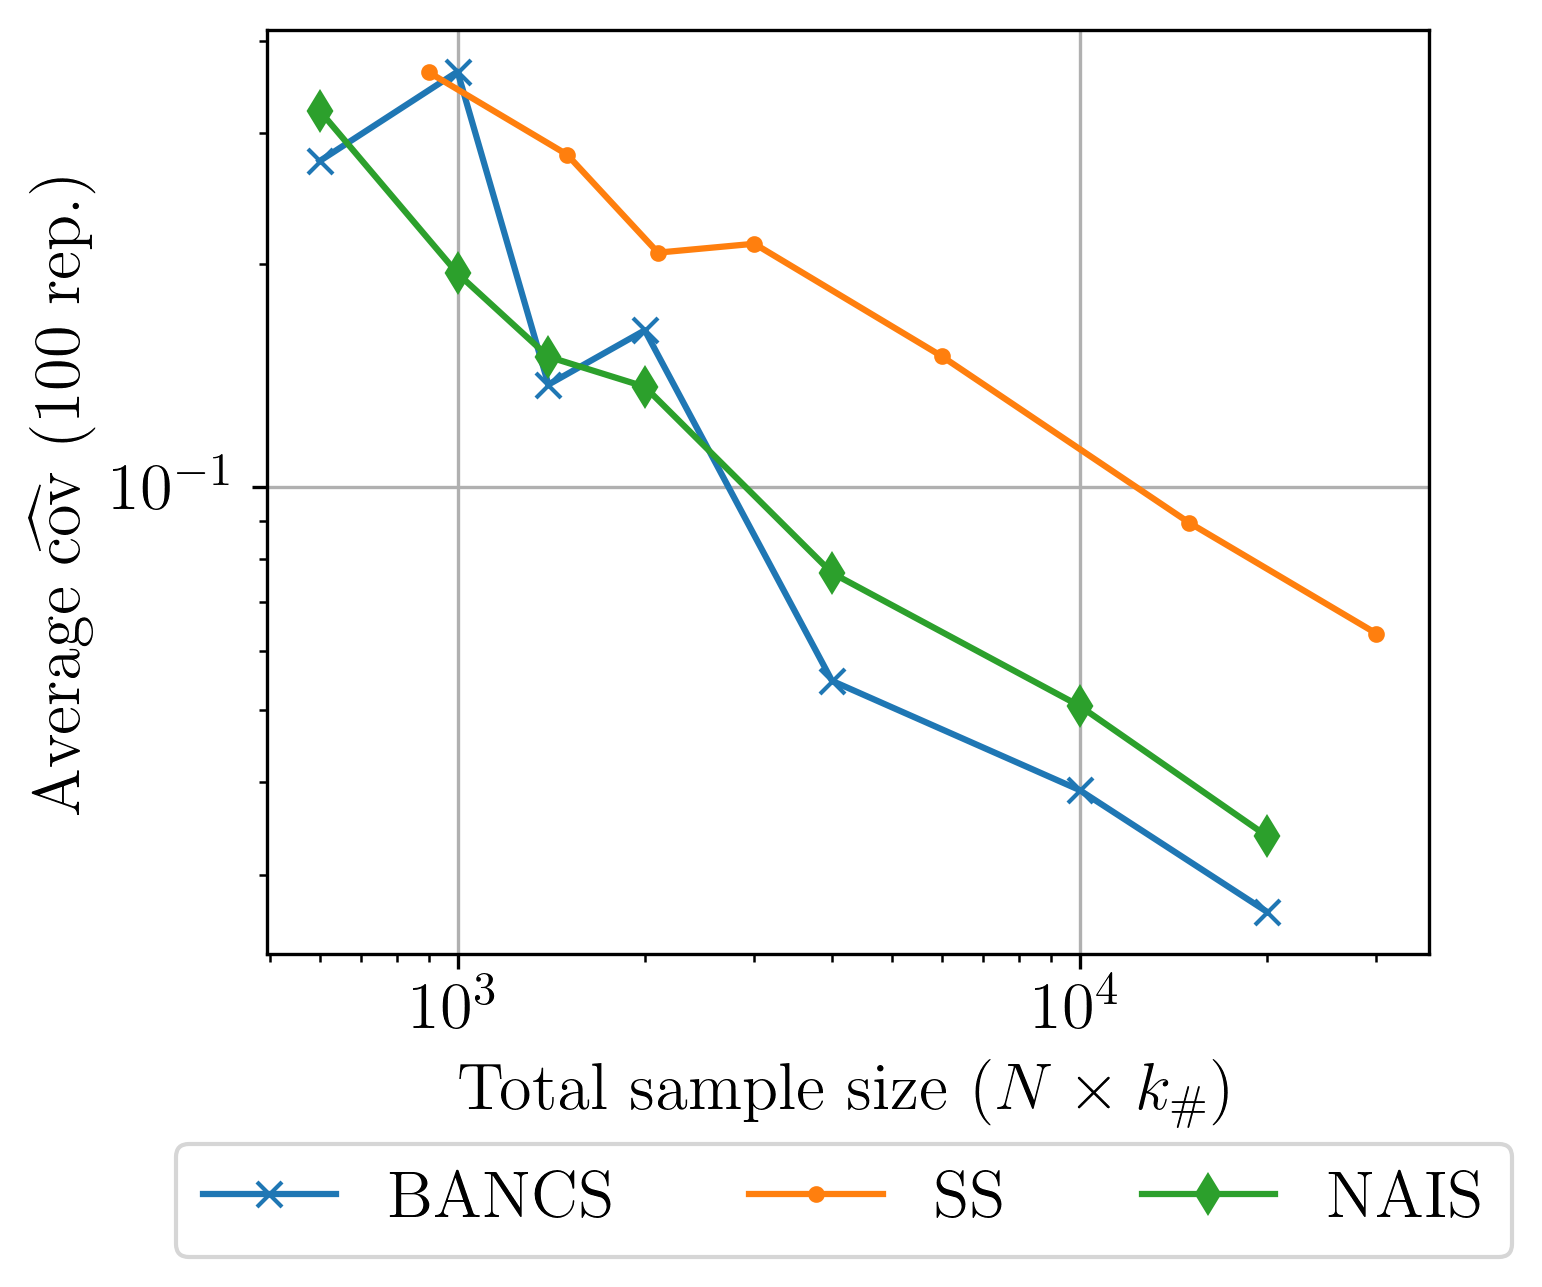
\includegraphics[width=\linewidth]{part3/figures/BANCS/RP38_cov.png}
        \caption{Coefficient of variation (toy-case \#4).}
    \end{subfigure}

    \begin{subfigure}[b]{0.49\linewidth}
        \centering
        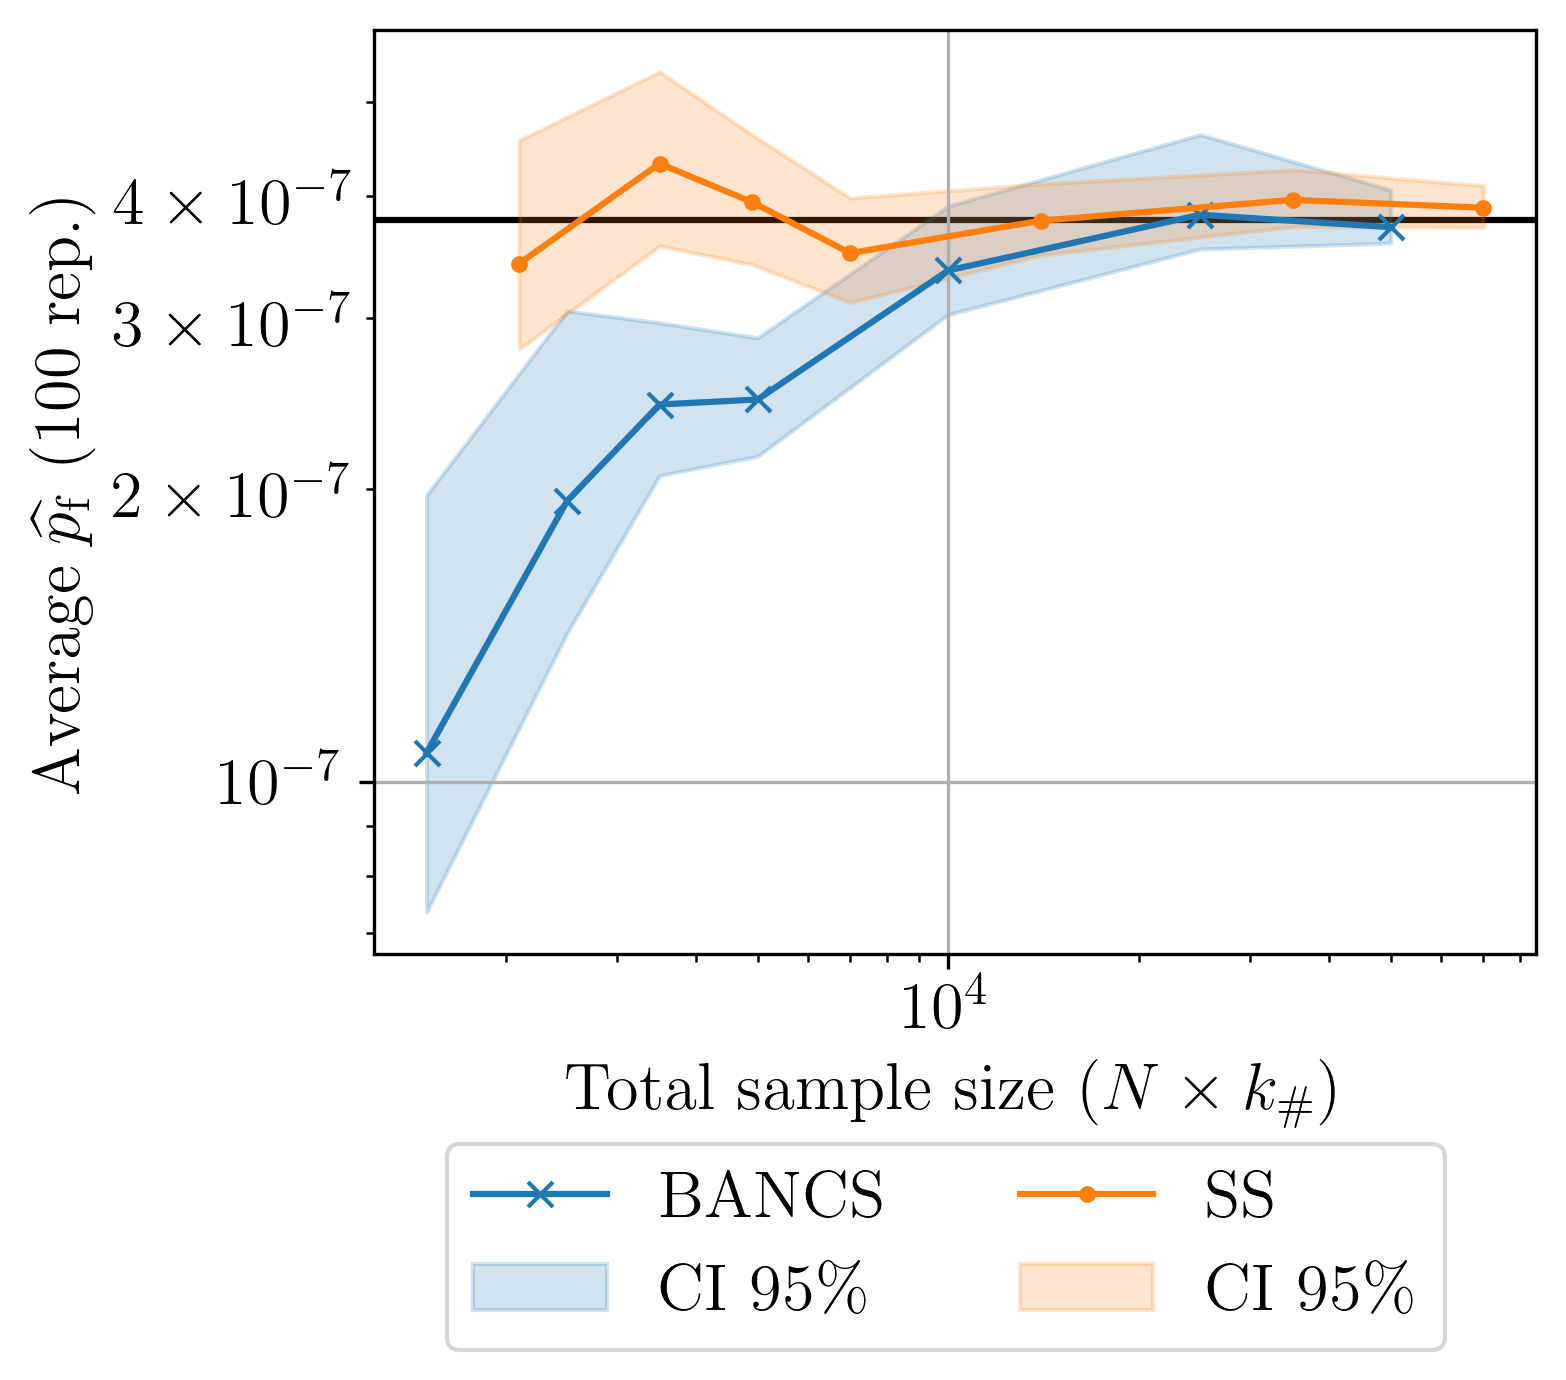
\includegraphics[width=\linewidth]{part3/figures/BANCS/Oscillator_mean.png}
        \caption{Failure probability (toy-case \#5).}
    \end{subfigure}
    \begin{subfigure}[b]{0.47\linewidth}
        \centering
        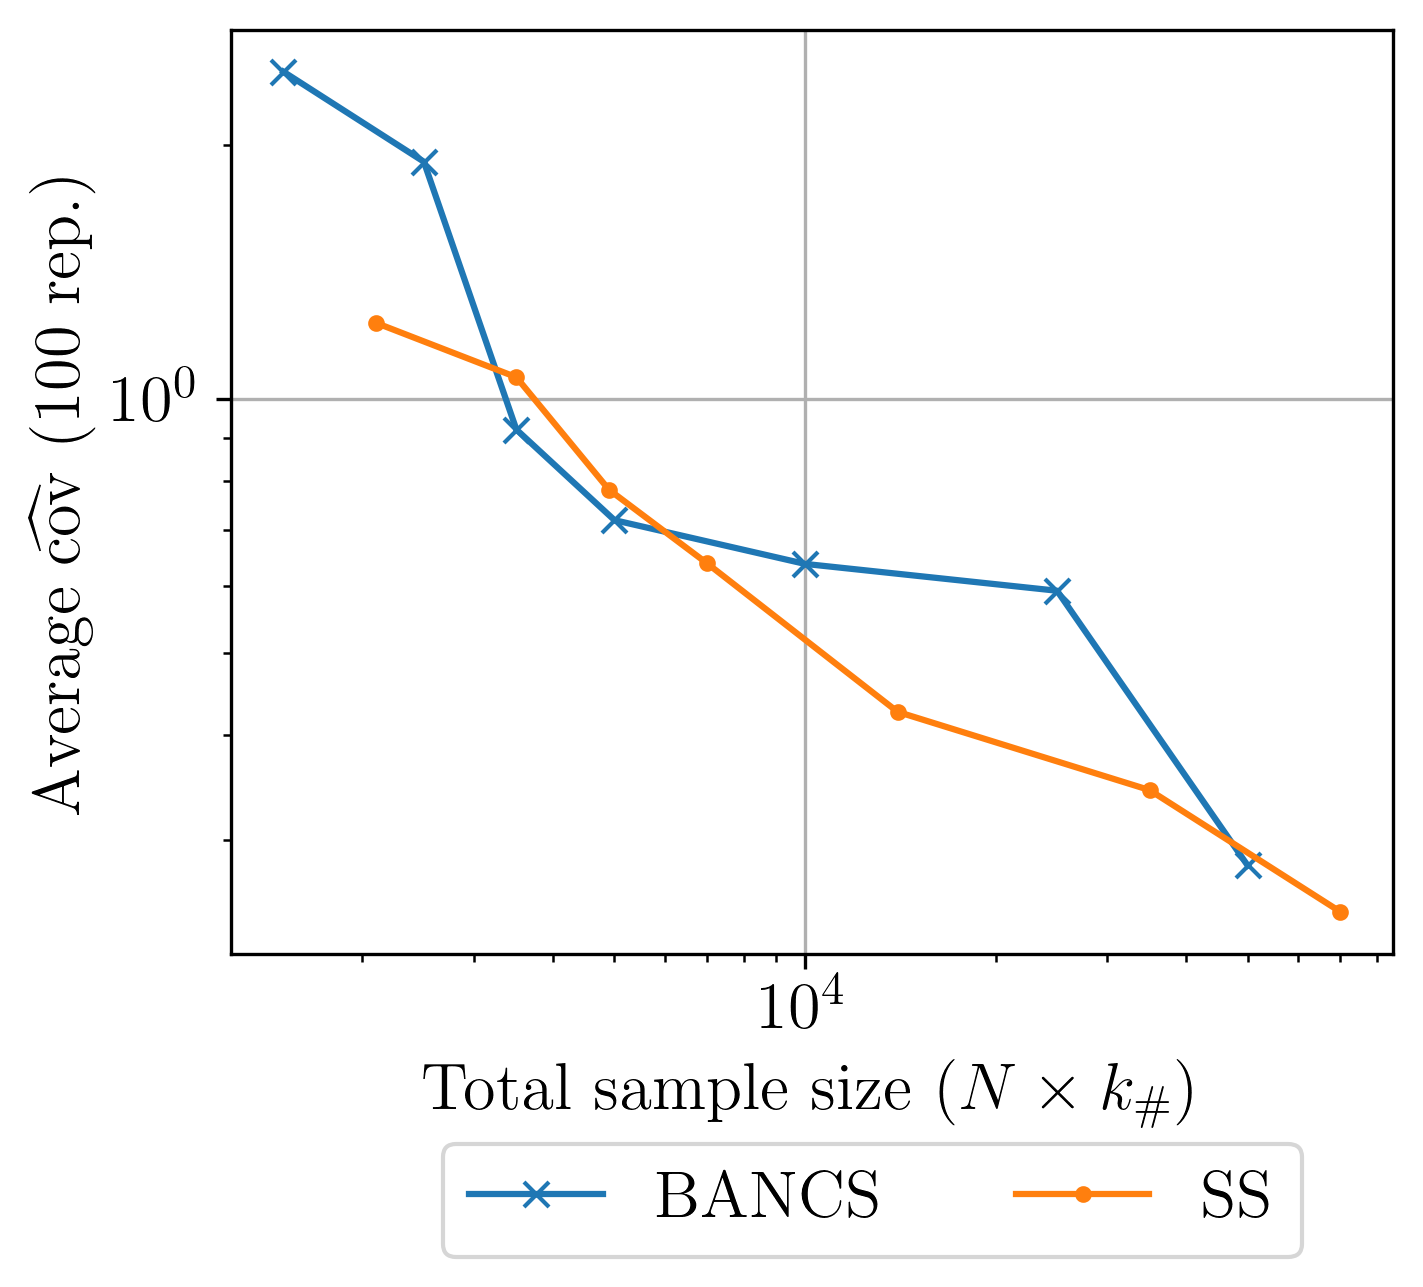
\includegraphics[width=\linewidth]{part3/figures/BANCS/Oscillator_cov.png}
        \caption{Coefficient of variation (toy-case \#5).}
    \end{subfigure}
    \caption{Reliability analysis benchmark between BANCS, SS and NAIS using 100 repetitions of each experiment (with $p_0=0.1$ for every methods). 
                The confidence intervals are obtained by Bootstrap on the repetitions. 
                The reference failure probabilities are represented by the horizontal black lines.}
    \label{fig:bancs_benchmark}
\end{figure}

%============================================================%
%============================================================%
\section{Reliability-oriented sensitivity analysis}\label{sec:bancs_rosa}
%============================================================%
%============================================================%

Global sensitivity analysis was introduced in Section~\ref{sec:gsa} as a tool to study the general impact of the input random variables on the output random variable. 
When estimating quantities of interest related to the output distribution's tail (e.g., failure probabilities), the SA should be dedicated to the subdomain of interest (i.e., failure domain). 
In other words, the global influence of the inputs (e.g., on the output's variance) may be different from their reliability-oriented influence (e.g., their influence on a rare event probability). 

To address the topic of \textit{reliability-oriented sensitivity analysis} (ROSA), different SA methods were adapted to the analysis of risk measures. 
The importance factors are a first local ROSA measure, near the most-probable failure point, obtained as a post-processing of FORM. 
Later on, global sensitivities such as the Sobol' indices were adapted to the indicator \citet{wei_2012_rosa,chabridon_2018_thesis,perrin_2019_rosa}. 
Recently, \citet{papaioannou_2021_rosa_form} discussed the link between the importance factors and the Sobol' indices on the indicator. 
Moment-independent importance measures were also applied to study the sensitivity of reliability. 
For example, \citet{daveiga_2015} suggested the use of Hilbert-Schmidt indepencence criterion (HSIC) for reliability which was further explored by \citet{marrel_chabridon_2021} who distinguished two categories of ROSA with different purposes: 
\begin{itemize}
    \item \textit{Target sensitivity analysis} (\abv{tsa}), measuring the influence of input variables to reach a restricted domain defined by the output (e.g., failure domain);
    \item \textit{Conditional sensitivity analysis} (\abv{csa}), studying the impact of input variables within the restricted domain (i.e., conditionally to this domain).
\end{itemize}
In the context of dependent inputs, the Shapley effects were adapted to the indicator function \citep{ilidrissi_2021_rosa,demange_2023_ijuq}. 

This section aims at demonstrating the estimation of TSA and CSA indices as a simple post-processing of BANCS. 
After estimating a rare event probability with BANCS, a set of i.i.d. samples (each with size $N$) is available. 
These consecutive samples gradually move closer to the failure domain and become rarer from the perspective of the initial input distribution. 
This section first recalls the TSA and CSA adaptation from \citet{marrel_chabridon_2021} of the Hilbert-Schmidt independence criterion (HSIC), a kernel-based sensitivity measure introduced in Section~\ref{sec:gsa} for GSA.
Then, the computation of the target-HSIC (respectively conditional-HSIC) is presented as a post-precessing of the BANCS reliability analysis of test-cases \#3 and \#5. 


%============================================================%
\subsection{Target and conditional HSIC}
%============================================================%

A first approach for TSA is to directly apply any SA measure to the binary variable $\1_{\{g(\bX) \leq \yth\}} = \1_{\{Y \leq \yth\}}$. 
This strategy does not distinguish points in the vicinity of the limit-state function from points far from this border. 
In the present work, a threshold relaxation using the weight transformation from \citet{marrel_chabridon_2021} is applied to gather more information. 
Let us consider the weight function $w_{\iF}: \R \rightarrow [0, 1]$ such that $w_{\iF}(y) = \exp(-d_{\iF}(y)/s)$, where $d_{\iF} = \mathrm{inf}_{y'\in \iF} \Vert y -y' \Vert$ is a distance to the border and $s\in\R$ is a smoothing parameter. 

Then, a TSA measure can be defined as the result of any sensitivity measure applied between the random inputs $\bX$ and $w_{\iF}(Y)$. 
In our case, the target-HSIC (T-HSIC) and their respective normalized version the target $R^2_{\HSIC}$ are defined as: 
\begin{subequations}
    \begin{align}
        T \mhyphen \HSIC(X_j, Y) & = \HSIC(X_j, w_{\iF}(Y)) = \MMD^2(\P_{(X_j, w_{\iF}(Y))}, \P_{X_j} \otimes \P_{w_{\iF}(Y)})\, ,\\
        T \mhyphen R^2_{\HSIC}(X_j, Y) &= \frac{T \mhyphen \HSIC(X_j, w_{\iF}(Y))}{\sqrt{T \mhyphen \HSIC(X_j, X_j) \, T \mhyphen \HSIC(w_{\iF}(Y), w_{\iF}(Y))}}\, .
    \end{align}
\end{subequations}
The stronger the dependence, the more $X_j$ is influent on the occurrence of the rare event $\{Y\in\iF\}$.  
Another advantage of applying the threshold relaxation is that any real-value kernel can be used to define the HSIC. 


To define the CSA indices, let us define the probability of $Y$ conditionally to the rare event $\{Y \in \iF\}$, considering the measurable space $(\Omega, \iA)$:
\begin{equation}
    \P_{Y|\{Y\in\iF\}}(A) = \frac{\int_{A} \1_{g(\bX)\leq0}(y) \, \dd \P_Y}{\pf}\,, \quad \forall A \in \iA\,.
\end{equation}
After applying the same threshold relaxation as earlier, one can write: 
\begin{equation}
    \P_Y^{w_{\iF}}(A)= \frac{\int_A w_{\iF}(y) \, \dd \P_Y}{\int_{\Omega} w_{\iF}(y) \, \dd \P_Y} \, ,
\end{equation}
and the conditional expectation: 
\begin{equation}
    \E[Y|Y \in \iF] = \E_{Y\sim\P_Y^{w_{\iF}}}[Y] = \frac{\int_\Omega y w_{\iF}(y) \, \dd \P_Y}{\int_{\Omega} w_{\iF}(y) \, \dd \P_Y}\, .
\end{equation}
Using this expression, the following conditional HSIC is developped in \citet{marrel_chabridon_2021}:
\begin{subequations}
    \begin{align}
        C \mhyphen \HSIC(X_j, Y) & = \HSIC_{(X_j, Y) \,\sim\, \P_{(X_j, Y)}^{w_{\iF}}} (X_j, w_{\iF}(Y)) \, ,\\
        C \mhyphen R^2_{\HSIC}(X_j, Y) &= \frac{C \mhyphen \HSIC(X_j, w_{\iF}(Y))}{\sqrt{C \mhyphen \HSIC(X_j, X_j) \, C \mhyphen \HSIC(w_{\iF}(Y), w_{\iF}(Y))}}\, .
    \end{align}
\end{subequations}

The R2-HSIC is a normalized index which can be used to rank variables by influence, but its value depends on the choice of kernel. 
Statistical tests are the only robust way of screening variables with respect to our quantity of interest. 
In the context of TSA, the asymptotic tests proposed by \citet{gretton_2006} are well suited to the sample sizes encountered in reliability analysis. 
However, the asymptotic approach no longer hold for CSA, which is replaced by the permutation-based statistical test proposed by \citet{delozzo_2016_hsic_test}.
Note that the HSIC generally do not require independence of the samples but the permutation tests do. 

The respective estimators of all indices are provided in \citet{marrel_chabridon_2021} and their implementation is available in \texttt{OpenTURNS}.
Unlike Sobol' indices, the HSIC estimation is realized on the same sample for every variable $X_j$. 
This property allows us to apply HSIC TSA and CSA to the samples evaluated during the BANCS reliability analysis.


%============================================================%
\subsection{ROSA as a post-processing of BANCS reliability analysis}
%============================================================%

After assessing a rare event probability using BANCS, a nested set of samples moving towards the failure domain is available.
This setup is the opportunity to study the evolution of the ROSA as the problem gets rarer.
At iteration $k$, a TSA is conducted on the sample $S_k$ with the intermediary threshold $\what{q}^{p_0}_k$ to study which random variables lead below this threshold. 
Then the CSA is assessed on the sample $S_{k+1}$, drawn according to the distribution $\what{f}_{[k+1]}$ which is conditional to the threshold $\what{q}^{p_0}_k$. 

The target and conditional sensitivity analysis are presented via their respective HSIC and the p-value of their independence test.  
These quantities are plotted as function of the consecutive samples $S_k$ to study the ROSA evolution. 
\fig{fig:rosa_ishigami} represents these results for the test-case \#3 while \fig{fig:rosa_oscillator} shows the results for test-case \#5. 
To ease the interpretation, a variable without any relation to the output was added. 
This variable always follows a standard normal distribution and is called the control variable (abbreviated ``ctrl.'' in the figures). 

%------------------------------------------------------------%
\paragraph{Test-case \#3:}
%------------------------------------------------------------%
On the Ishigami problem, the variable $X_2$ has the least influence on the TSA while the variable $X_3$ has the least influence on the CSA. 
The p-value obtained asymptotically for the TSA and by permutations for the CSA, confirm the interpretation of the HSICs. 
One can conclude that the three variables all have a distinct impact on the failure probability. 
The variable $X_1$ has an interesting behavior as the problem becomes rarer, its impact on the TSA decreases while its influence on the CSA increases.      
It is overall the most influential variable on this ROSA study.  

%------------------------------------------------------------%
\paragraph{Test-case \#5:}
%------------------------------------------------------------%
On the oscillator problem, the variables $F_s, \zeta_s$, and $\zeta_p$ have a high target HSIC and low target p-value, meaning that they lead to the failure domain.    
Interestingly, the T-HSIC and C-HSIC of the resistance variable $F_s$ decrease as the problem becomes rarer. 
However, $F_s$ remains of prime importance on the CSA. 
On this medium dimension problem, the variables $m_p$ and $k_s$ have among the lowest T-HSIC. 

A similar study was conducted on this test-case by \citet{bourinet_2018} using local ROSA measures, called the score-functions, which rely on derivatives of the failure probability with respect to the moments of the inputs. 
The results from this work, based on consecutive samples from a subset simulation, are reproduced in \fig{fig:score_functions_oscillator}. 
Considering a subset probability $p_0$, the nested failure probabilities are denoted by $\pi_s = \Pi_{k=1}^s p_0$, and the inputs first moments by $(\mu_i, \sigma_i)$. 

Variables with score-function close to zero should have a small influence on the reliability. 
Then, one can notice that the conclusions of this local ROSA are quite in line with the target HSIC. 
The consequence of fixing these variables to their mean values should be further studied to propose solid recommendations for screening in ROSA.


\begin{figure}
    \centering
    \begin{subfigure}[b]{0.48\linewidth}
        \centering
        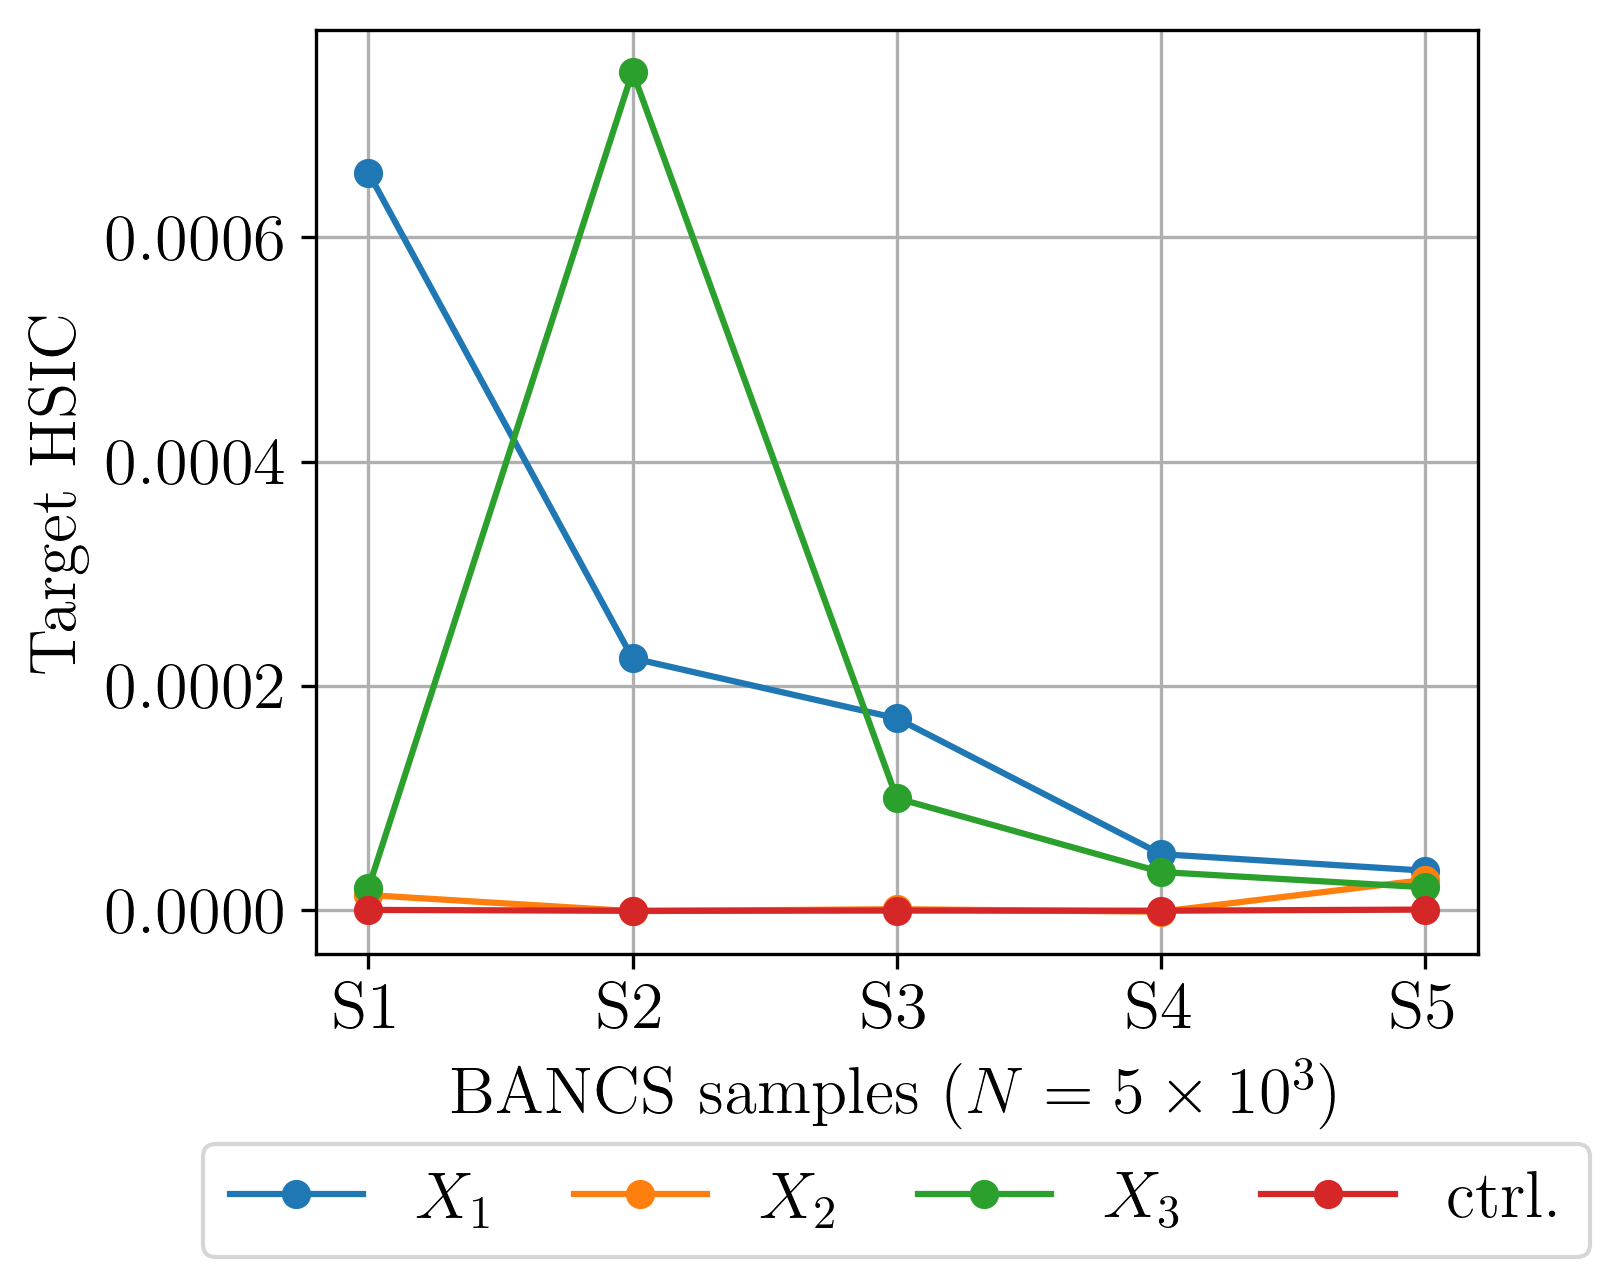
\includegraphics[width=\linewidth]{part3/figures/BANCS/ishigami_THSIC.png}
        \caption{Target $\HSIC(X_j, Y)$.}
    \end{subfigure}
    \begin{subfigure}[b]{0.48\linewidth}
        \centering
        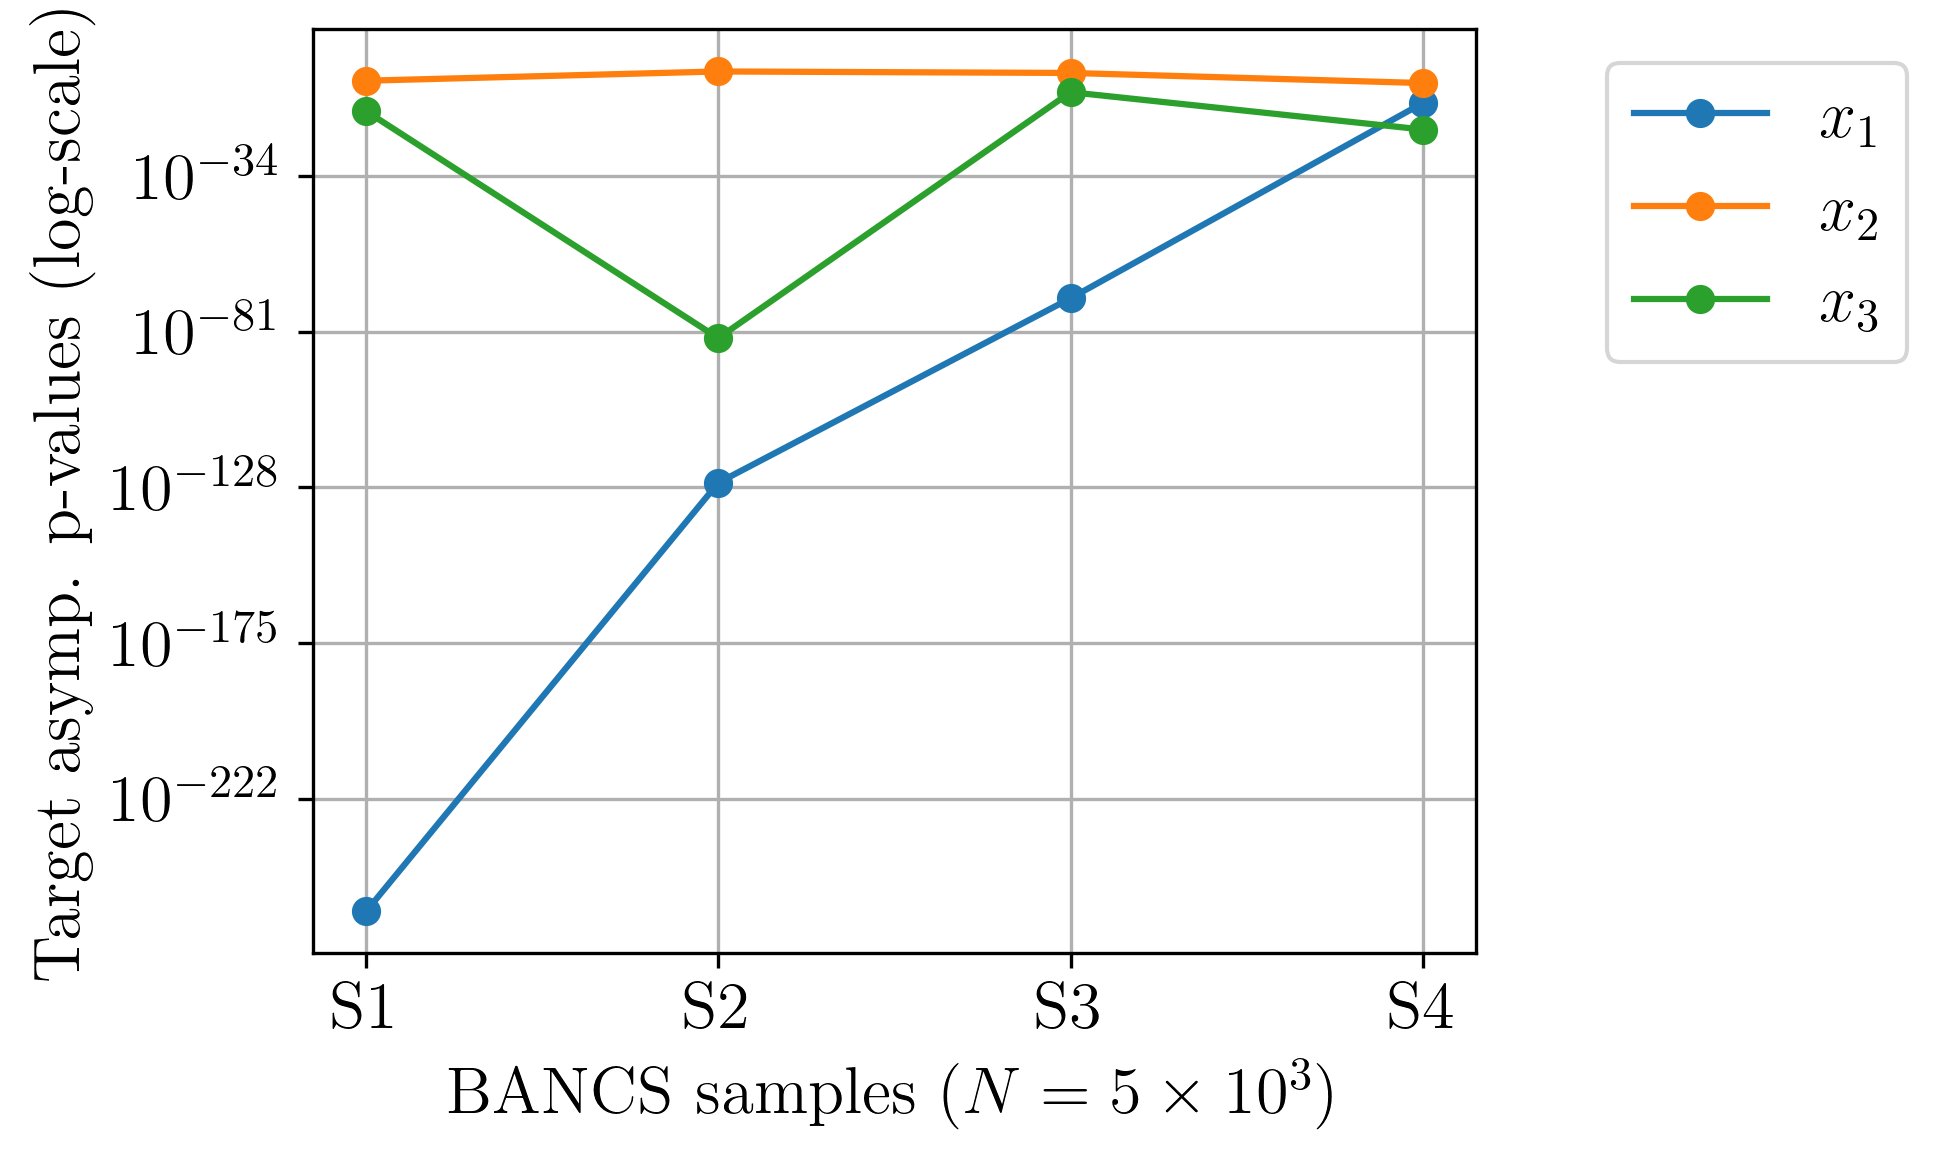
\includegraphics[width=\linewidth]{part3/figures/BANCS/ishigami_Tpvalue_asymptotic.png}
        \caption{Target asymptotic p-value.}
    \end{subfigure}
    \\[20pt]
    \begin{subfigure}[b]{0.48\linewidth}
        \centering
        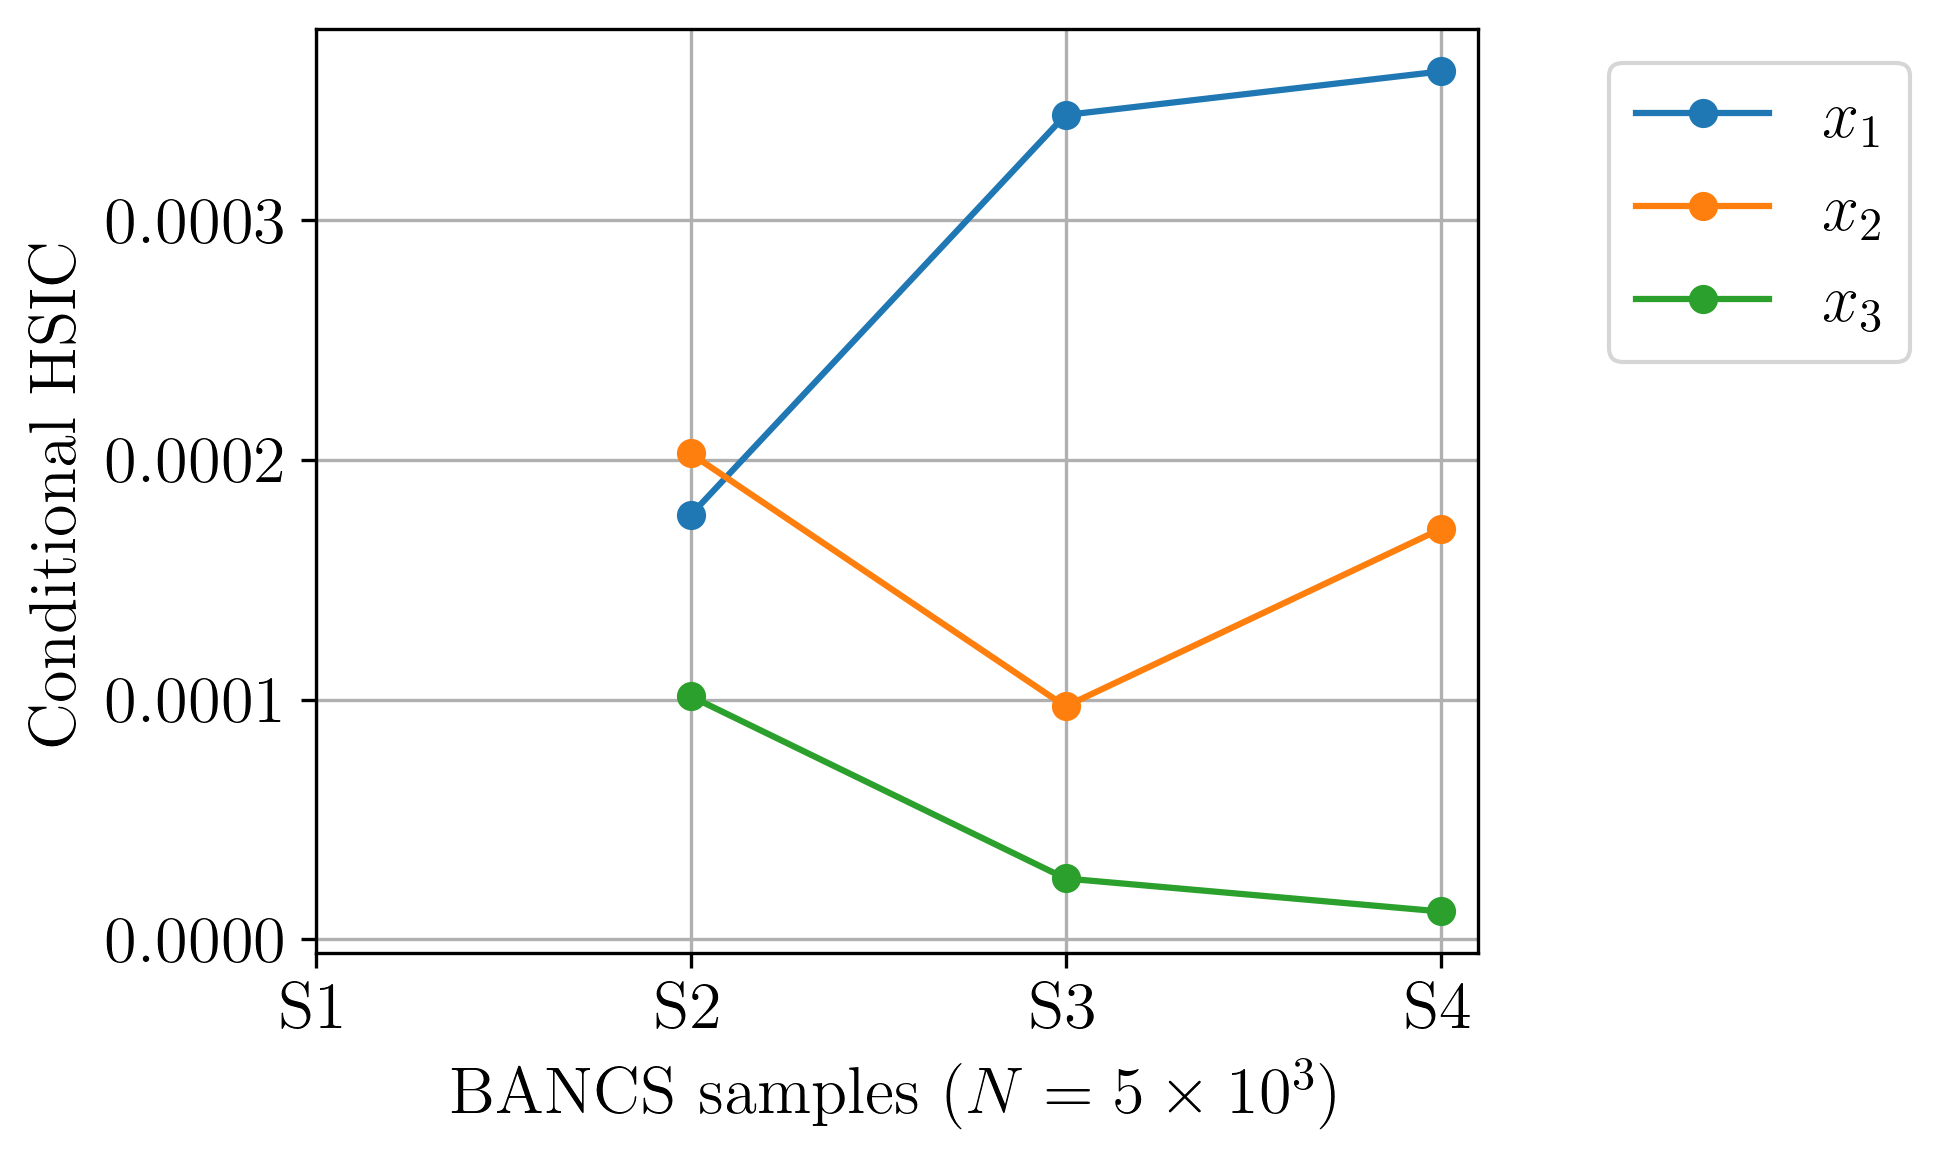
\includegraphics[width=\linewidth]{part3/figures/BANCS/ishigami_CHSIC.png}
        \caption{Conditional $\HSIC(X_j, Y)$.}
    \end{subfigure}
    \begin{subfigure}[b]{0.48\linewidth}
        \centering
        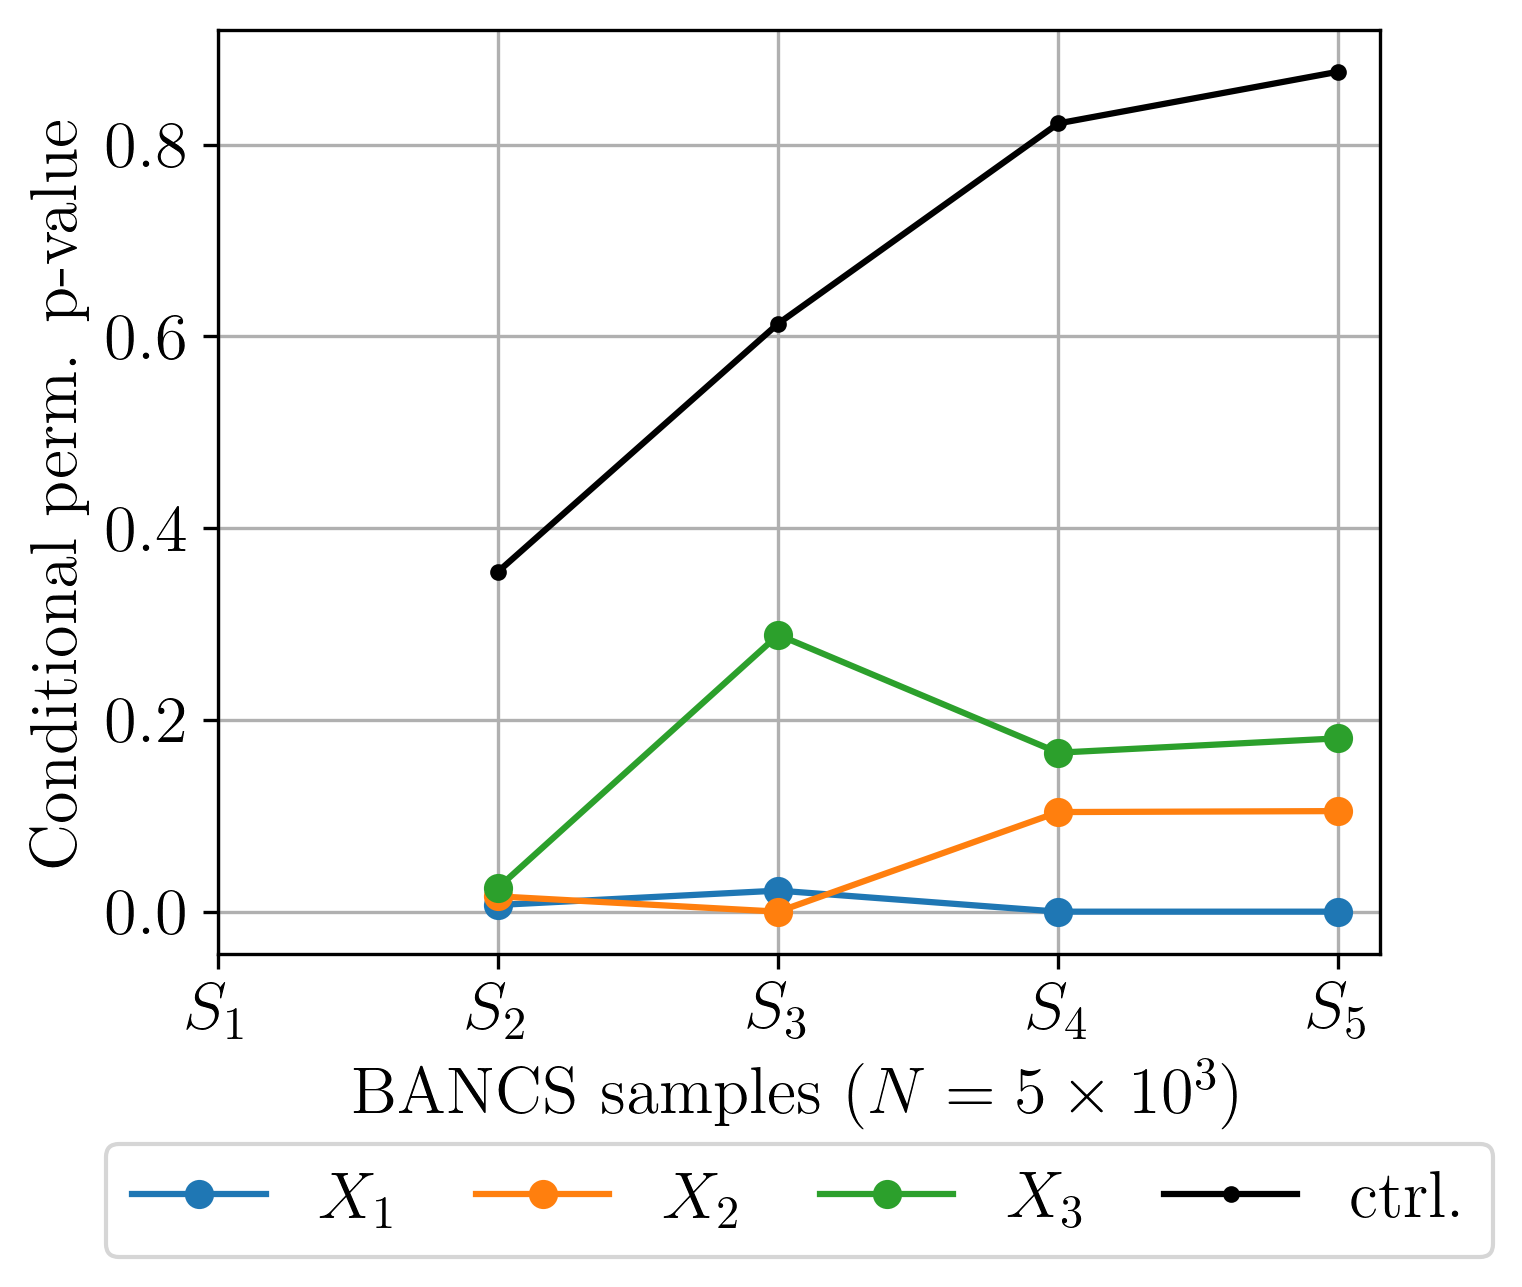
\includegraphics[width=\linewidth]{part3/figures/BANCS/ishigami_Cpvalue_permutation.png}
        \caption{Conditional p-value by perm. ($10^3$ perm.).}
    \end{subfigure}
    \caption{Target and conditional HSIC as a post-processing of BANCS reliability analysis of test-case \#3 (modified Ishigami). 
                The consecutive samples from BANCS are denoted by $\{S_k\}_{k=1}^{k_\#}$ (each with size $N=5\times10^3$, with $p_0=0.25$).}
    \label{fig:rosa_ishigami}
\end{figure}


\begin{figure}
    \centering
    \begin{subfigure}[b]{0.48\linewidth}
        \centering
        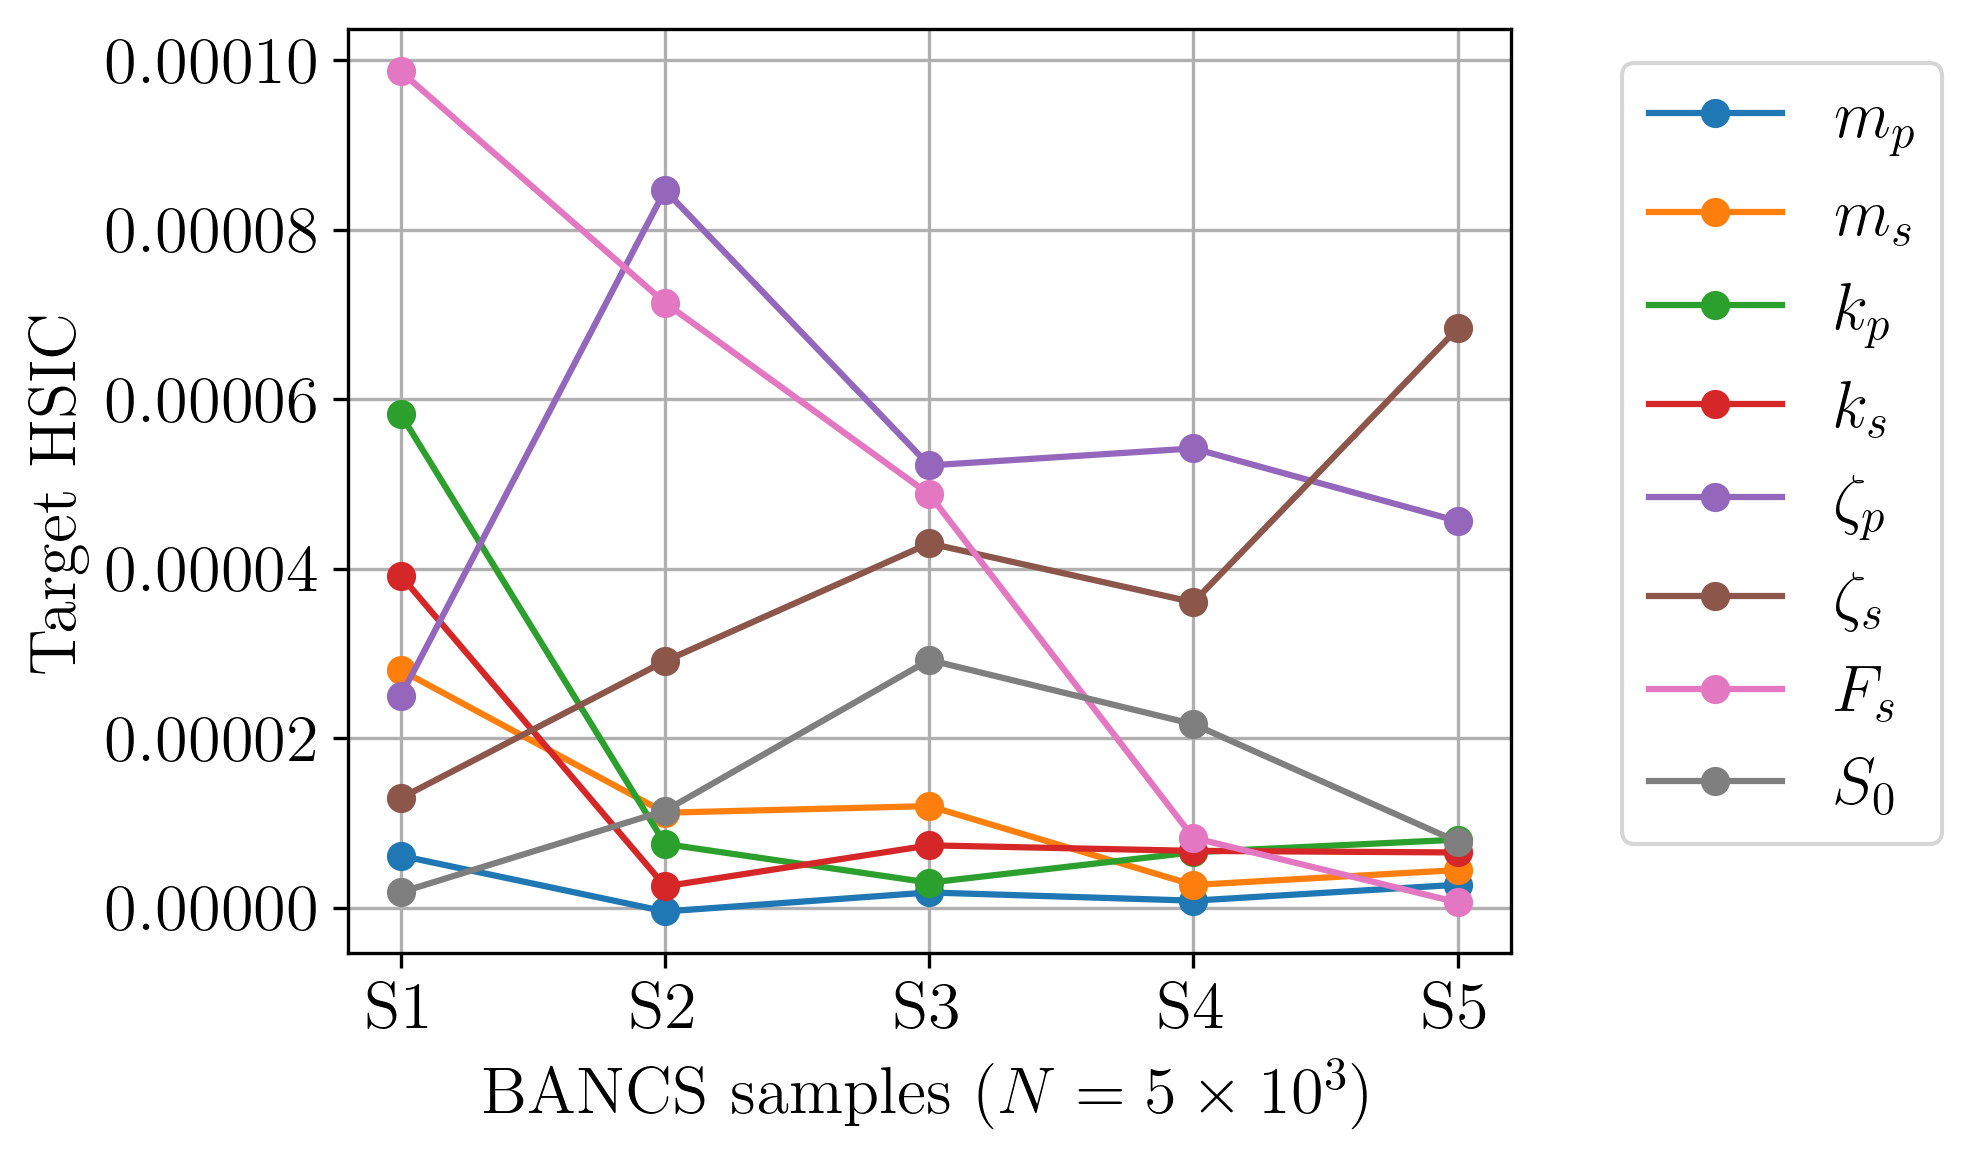
\includegraphics[width=\linewidth]{part3/figures/BANCS/oscillator_THSIC.png}
        \caption{Target $\HSIC(X_j, Y)$.}
    \end{subfigure}
    \hfill
    \begin{subfigure}[b]{0.48\linewidth}
        \centering
        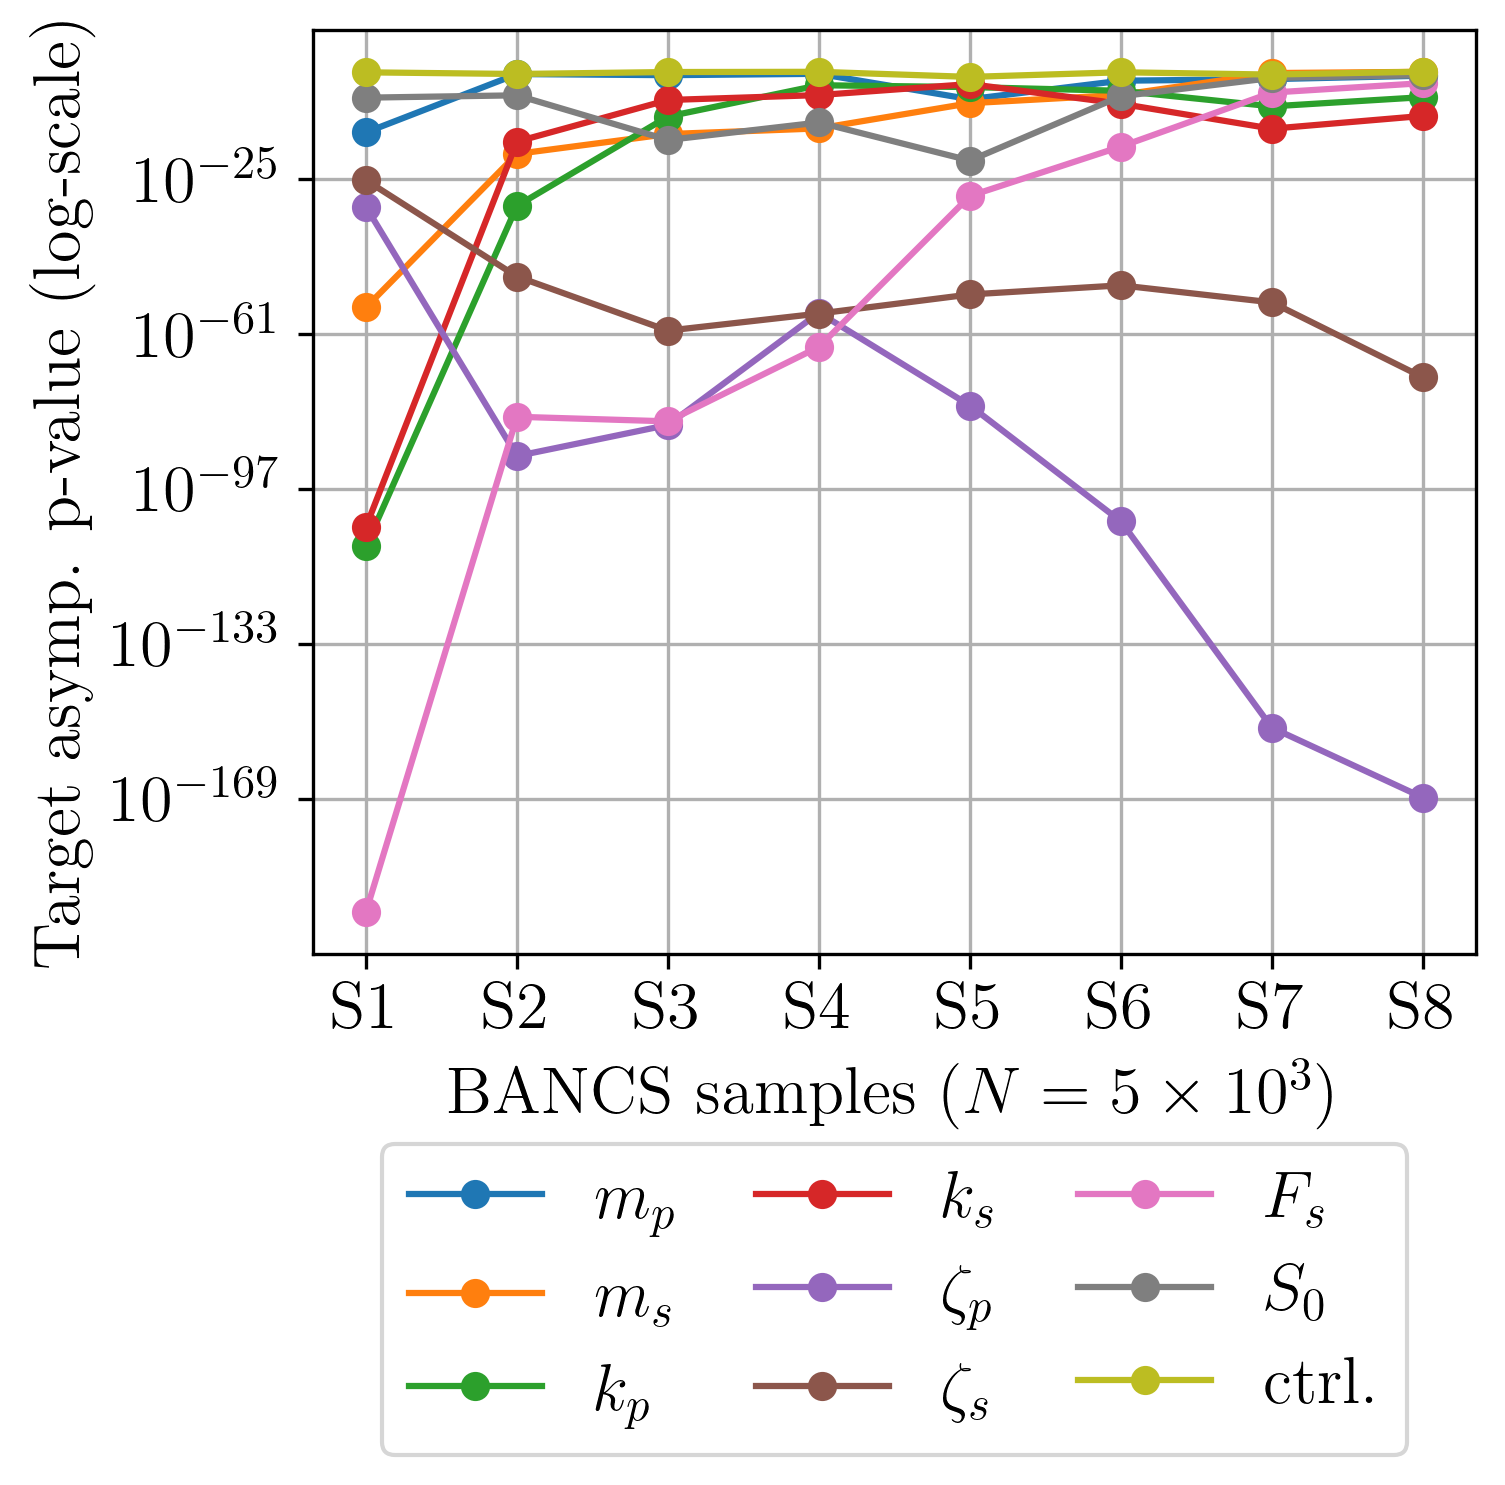
\includegraphics[width=\linewidth]{part3/figures/BANCS/oscillator_Tpvalue_asymptotic.png}
        \caption{Target asymptotic p-value.}
    \end{subfigure}
    \\[20pt]
    \begin{subfigure}[b]{0.48\linewidth}
        \centering
        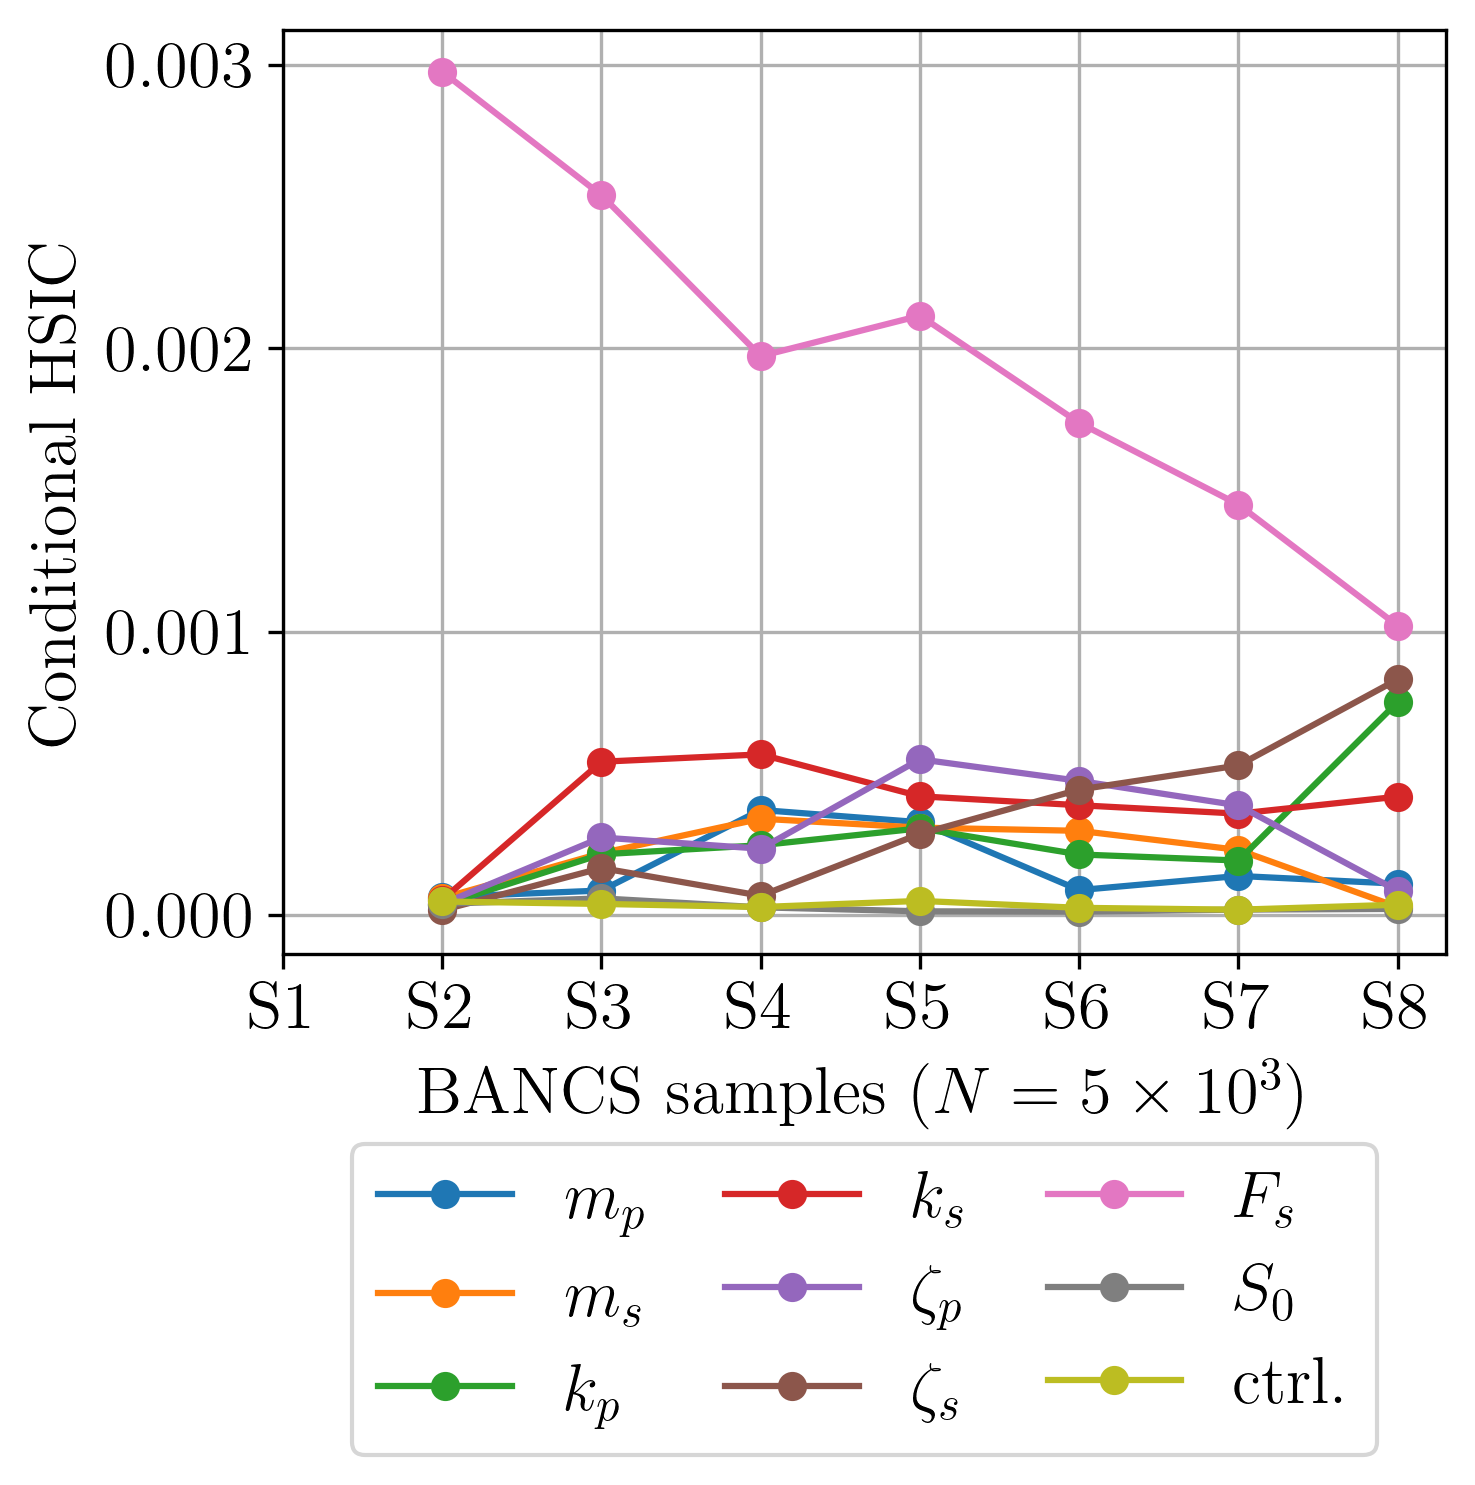
\includegraphics[width=\linewidth]{part3/figures/BANCS/oscillator_CHSIC.png}
        \caption{Conditional $\HSIC(X_j, Y)$.}
    \end{subfigure}
    \hfill
    \begin{subfigure}[b]{0.48\linewidth}
        \centering
        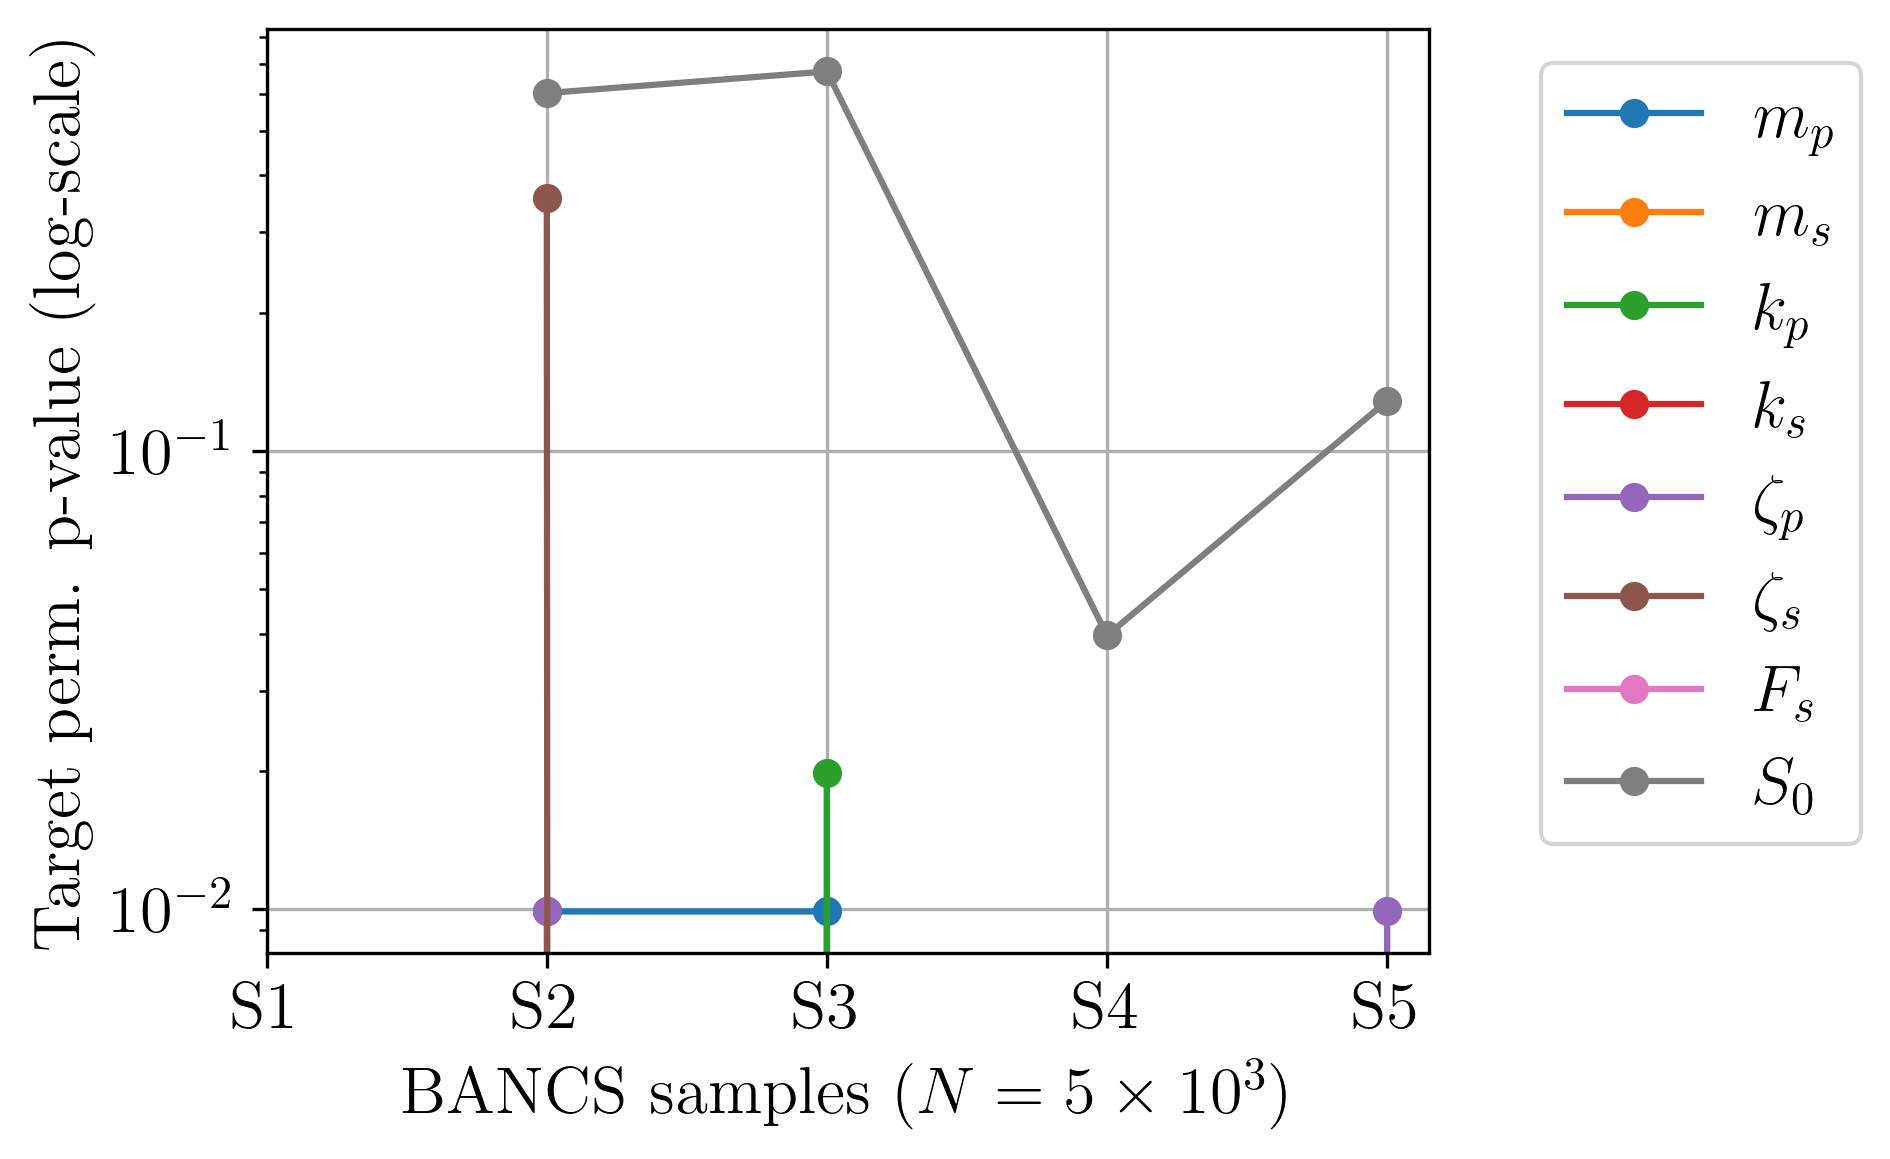
\includegraphics[width=\linewidth]{part3/figures/BANCS/oscillator_Cpvalue_permutation.png}
        \caption{Conditional p-value by perm. ($10^3$ perm.).}
    \end{subfigure}
    \caption{Target and conditional HSIC as a post-processing of BANCS reliability analysis of test-case \#5 (oscillator problem). 
    The consecutive samples from BANCS are denoted by $\{S_k\}_{k=1}^{k_\#}$ (each with size $N=5\times10^3$, with $p_0=0.25$).}
    \label{fig:rosa_oscillator}
\end{figure}


\begin{figure}
    \centering
    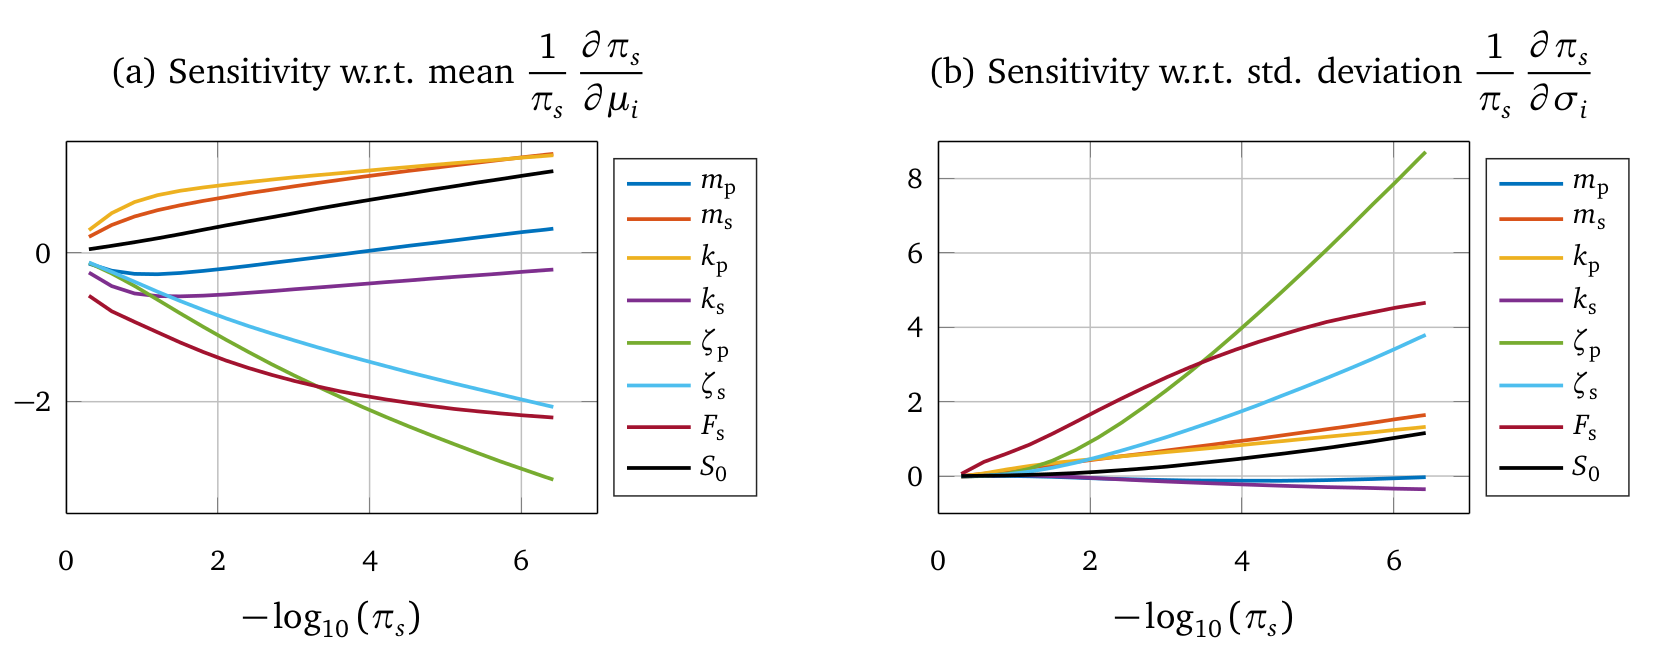
\includegraphics[width=0.9\linewidth]{part3/figures/BANCS/score_function_HDR_JMB.png}
    \caption{Normalized score-functions of $\pi_s = \Pi_{k=1}^s p_0$ w.r.t. the inputs mean $\mu_i$ and standard deviation $\sigma_i$ in the standard normal space (source: \citealp[p.54]{bourinet_2018}). 
            The consecutive probabilities result from a subset simulation (with $N=10^6$ and $p_0=0.5$ per subset).}
    \label{fig:score_functions_oscillator}
\end{figure}



%============================================================%
%============================================================%
\section{Conclusion}
%============================================================%
%============================================================%

In this chapter a contribution to rare event estimation was presented. 
BANCS is a new adaptive importance sampling method using nonparametric Bernstein copula to fit the successive conditional distributions. 
Its performance was compared in a numerical benchmark with other methods as SS and NAIS. 
The current implementation is at least as efficient as the other methods on the analytical problems studied, however numerous potential improvement remain unexplored. 
A first perspective lies in the optimization of the EBC polynomial order by applying a validation procedure similar what is done for surrogate models (among the elite set, a test set could be selected using the results from Chapter~\ref{chpt:5}). 
Then, instead of estimating the intermediary quantiles by Monte Carlo, other sampling methods could be tested (e.g., LHS, randomized QMC, see \citealp{tuffin_2019}, or importance sampling including all the samples). 
To tackle high-dimentional problems, the inference of copulas by blocks could be interesting (see e.g., \citealp{lasserre_2022}).

BANCS also presents multiple advantages, first, it does not require a transformation in the standard space, second, its flexibility allows capturing multimodal problems. 
A third advantage is that the samples generated at each iteration are i.i.d., offering the possibility to assess global reliability-oriented sensitivity analysis as a post-processing. 
In this chapter, the ROSA was investigated using the HSIC (in the vein of the work of \citealp{marrel_chabridon_2021}) but the use of Shapley indices could provide tools for understanding problems with dependent inputs \citep{ilidrissi_2021_rosa}.
This complementary analysis is an essential tool to understand the influence of the inputs on the failure probability. 
Further studies should be conducted to guarantee the screening of noninfluential variables in the context of rare events. 


%\begin{itemize}
%    \item Compare the learning-time with NAIS
%    \item Perspective learning the entire distribution with Bernstein polynomials
%    \item learning the copula by blocks to tackle high-dimensional problems
%    \item Estimate the quantiles with IS on all previous samples
%    
%    \item Advantage of working directly in the physical space directly
%    \item We could fit the marginals with parametric models and compare
%\end{itemize}